\documentclass[a4paper]{article}
\usepackage{tikz, pgfplots}
\usepgfplotslibrary{groupplots,units}
\pgfplotsset{compat=1.15}
\usepackage{float}
\usepackage{lscape}
\usepackage{array}
\usepackage[nottoc,numbib]{tocbibind}
%\addcontentsline{toc}{section}{References}
\usepackage{multirow}
\usepackage{tikz}
\usepackage{cite}
\usepackage{circuitikz}
\usepackage{mathtools}
\usepackage{mleftright}
\usepackage{physics}
\usetikzlibrary{shapes.geometric, arrows}
\usepackage{url}
% \usepackage[hidelinks]{hyperref}
% \usepackage[utf8]{inputenc}
% \usepackage[T1]{fontenc}
% \usepackage[english]{babel}
% \usepackage{alphabeta}
\usepackage{fancyhdr} % Required for custom headers
\usepackage{lastpage} % Required to determine the last page for the footer
\usepackage{extramarks} % Required for headers and footers
% \usepackage{graphicx} % Required to insert images
% \usepackage{amsmath,amssymb,amsthm,amsfonts}
% \usepackage{cleveref}
% \usepackage{commath}
% \usepackage{caption}
% \usepackage{subcaption}
% \setlength{\parindent}{4em}
% \setlength{\parskip}{1em}
% \usepackage{listings}
% \usepackage{bm}
% \usepackage{gensymb}
% \usepackage{color} %red, green, blue, yellow, cyan, magenta, black, white

% \usepackage[iso-8859-7]{inputenc}
\usepackage{gfsdidot}
\usepackage[T1]{fontenc}
\usepackage[utf8]{inputenc}
\usepackage[english,greek]{babel}
\usepackage{amsmath,amsfonts,amssymb}
\usepackage[parfill]{parskip}
\usepackage[unicode]{hyperref}
% \usepackage{kmath,kerkis}
% \def\tl{\textlatin}
% \def\tg{\textgreek}
% \usepackage{helvet}
% \renewcommand{\familydefault}{\sfdefault}

\tikzstyle{startstop} = [rectangle, rounded corners, minimum width=3cm, minimum height=1cm,text centered, draw=black, fill=red!30]

\tikzstyle{io} = [trapezium, trapezium left angle=70, trapezium right angle=110, minimum width=3cm, minimum height=1cm, text centered, text width=2.5cm, draw=black, fill=blue!30]

\tikzstyle{process} = [rectangle, minimum width=3cm, minimum height=1cm, text centered, text width=4cm, draw=black, fill=orange!30]

\tikzstyle{decision} = [diamond, minimum width=3cm, minimum height=1cm, text centered, draw=black, fill=green!30]

\tikzstyle{arrow} = [thick,->,>=stealth]

\tikzstyle{arrow2} = [thick,-,>=stealth]

\tikzstyle{output} = [coordinate]
% Margins
\topmargin=-0.45in
\evensidemargin=0in
\oddsidemargin=0in
\textwidth=6.3in
\textheight=9.6in
\headsep=0.25in

%\linespread{1.1} % Line spacing

\setlength\parindent{0pt} % Removes all indentation from paragraphs

%\setcounter{secnumdepth}{0} % Removes default section numbers

% Set up the header and footer


\renewcommand\headrulewidth{0.4pt} % Size of the header rule
%\renewcommand\footrulewidth{0.4pt} % Size of the footer rule



%	NAME AND CLASS SECTION
\newcommand{\hmwkTitle}{Modelling \& Design of a Prototype DC/DC Converter for Trip Coil Applications} % Assignment title
%\newcommand{\hmwkClass}{EG2330} % Course/class
%\newcommand{\hmwkClassName}{Power System Design Project Course} % Course/class

\usepackage{fancyhdr}

\pagestyle{fancy}
%\rfoot{Page\ \thepage\ of\ \pageref{LastPage}} % Bottom right footer

%\chead{Power-electronics system for grid-connected PV plants} % Top center header
\rhead{} % Top right header
% \cfoot{}
%	TITLE PAGE


\title{
	%\includegraphics[width=2in]{kth_cmyk_electr_engine.eps}\\
	%\vspace{1.5in}
	%\textmd{\textbf{\hmwkClass\ -- \hmwkClassName}}\\
	%\vspace{0.2in}
	\textmd{\textbf{\hmwkTitle}}\\
%	\normalsize\vspace{0.1in} \small{\today}\\
	\vspace{2in} 
}
\author{
\textbf{\Large{Orestis Apostolou}}\\
}


\date{February 2021}

\usepackage{afterpage}

\newcommand\blankpage{%
    \null
    \thispagestyle{empty}%
    \addtocounter{page}{-1}%
    \newpage}
    
\begin{document}
\afterpage{\blankpage}
\begin{titlepage}
    \begin{center}
        \vspace*{4cm}
        \huge
        \rmfamily
        \textbf{Σχεδιασμός και Κατασκευή Εφαρμογής Τεχνητής Νοημοσύνης για την Πρόγνωση της Στεφανιαίας Νόσου σε Περιβάλλον \selectlanguage{english}iOS \selectlanguage{greek}}
        
        \vspace{0.5cm}
        
        \vspace{1.5cm}
        \LARGE
        \textbf{Αποστόλου Ορέστης}
        
        \vfill
        \large 
        \begin{flushleft}
        \selectlanguage{greek}
        Τμήμα Ηλεκτρολόγων Μηχανικών και Μηχανικών Ηλεκτρονικών Υπολογιστών\\
        Αριστοτέλειο Πανεπιστήμιο Θεσσαλονίκης\\
        Θεσσαλονίκη, Ελλάδα\\
        Επιβλέπων Καθηγητής: Χαρίσης Βασίλειος\\
        Φεβρουάριος 2021
        \end{flushleft}
    \end{center}
\end{titlepage}

\pagenumbering{roman}	

    
    %\section{Περιληπτικά}

Η στεφανιαία καρδιακή νόσος, ή απλά στεφανιαία νόσος, είναι μια ασθένεια της καρδιάς. Προκαλείται από το φράξιμο των αθηρωματικών αρτηριών, με συνέπεια να εμποδίζεται η παροχή αίματος στην καρδιά. Αυτό, έχει ως αποτέλεσμα τη μειωμένη παροχή οξυγόνου και θρεπτικών ουσιών στους ιστούς της καρδιάς.

Η στεφανιαία νόσος είναι η πρωταρχική αιτία θανάτου στις σύγχρονες κοινωνίες, με ποσοστό 15.6\% επί των συνολικών θανάτων παγκοσμίως. Το 2015, επηρέασε 110 εκατομμύρια ανθρώπους, και προκάλεσε 8.9 εκατομμύρια θανάτους \cite{wikiCAD}.

Συνηθέστερη αιτία πρόκλησης της στεφανιαίας νόσου είναι η αθηροσκλήρωση, κατά την οποία δημιουργούνται αθηρωματικές πλάκες, οι οποίες επικάθονται στον αυλό των στεφανιαίων αρτηριών, δυσκολεύοντας έτσι τη φυσιολογική ροή του αίματος. Οι αθηρωματικές πλάκες σχηματίζονται από εναποθέσεις λίπους στις αρτηρίες, μια κατάσταση που ονομάζεται αρτηριοσκλήρυνση, και οδηγεί στην στένωση ή την απόφραξη των αγγείων. Η ρίξη της αθηρωματικής πλάκας ονομάζεται αθηροθρόμβωση και ακολουθείται από πλήρη και παρατεταμένη έλλειψη οξυγόνου στο μυοκάρδιο, που με τη σειρά του προκαλεί τη νέκρωση του μυοκαρδίου, γνωστή και ως έμφραγμα.

Παράγοντες οι οποίοι συνδέονται με αυξημένο κίνδυνο πρόκλησης στεφανιαίας νόσου είναι η υψηλή αρτηριακή πίεση, το κάπνισμα, ο διαβήτης, η έλλειψη άσκησης, η παχυσαρκία, η κατάθλιψη και η υπερβολική κατανάλωση αλκοόλ.

Οι συνηθέστεροι τρόποι διάγνωσης της στεφανιαίας νόσου είναι η στεφανιογραφία και το ηλεκτροκαρδιογράφημα. Η διάγνωση της στεφανιαίας νόσου κρίνεται ιδιαίτερα σημαντική, καθώς με τις κατάλληλες αλλαγές στον τρόπο ζωής, μπορούν να προληφθούν σε σημαντικό ποσοστό τα επικίνδυνα συμπτώματά της. \cite{abstract1, abstract2}

Εξαιτίας της σοβαρότητας αυτής της νόσου, τα τελευταία χρόνια έχουν γίνει πολλές προσπάθειες στον τομέα της βιοϊατρικής για να δημιουργηθούν αυτοματοποιημένοι και εύκολοι τρόποι διάγνωσης. Ανάμεσα σε αυτές, είναι και ορισμένοι έξυπνοι αλγόριθμοι τεχνητής νοημοσύνης (αναφορές θέλει εδώ), οι οποίοι χρησιμοποιούν συνήθως κάποιο ηλεκτροκαρδιογράφημα του ασθενή και προσπαθούν να διαγνώσουν εάν ο ασθενής έχει στεφανιαία νόσο. Ωστόσο, ως επί τω πλείστω, οι αλγόριθμοι αυτοί χρειάζονται ως είσοδο 
ένα ηλεκτροκαρδιογράφημα μεγάλης χρονικής διάρκειας (συνήθως 24ωρο), δυσκολεύοντας έτσι τη χρήση τους στην καθημερίνη ζωή.

Η παρούσα μελέτη, έχει ως σκοπό τη δημιουργία μιας ολοκληρωμένης εφαρμογής στο λειτουργικό σύστημα \selectlanguage{english}Apple iOS\selectlanguage{greek}, στην οποία ο χρήστης θα μπορεί να λαμβάνει ένα ή περισσότερα καρδιογραφήματα διάρκειας 30 δευτερολέπτων, και ο αλγόριθμος τεχνητής νοημοσύνης που έχει κατασκευαστεί να μπορεί να εμφανίζει την πιθανότητα εμφάνισης στεφανιαίας νόσου στον ασθενή.
    %\newpage
    
    \setcounter{page}{1}
    %\tableofcontents
    \newpage
\graphicspath{{Figures/}}
\setcounter{secnumdepth}{0}
\section{Περιληπτικά}

Η στεφανιαία καρδιακή νόσος, ή απλά στεφανιαία νόσος, είναι μια ασθένεια της καρδιάς. Προκαλείται από το φράξιμο των αθηρωματικών αρτηριών, με συνέπεια να εμποδίζεται η παροχή αίματος στην καρδιά. Αυτό, έχει ως αποτέλεσμα τη μειωμένη παροχή οξυγόνου και θρεπτικών ουσιών στους ιστούς της καρδιάς.

Η στεφανιαία νόσος είναι η πρωταρχική αιτία θανάτου στις σύγχρονες κοινωνίες, με ποσοστό 15.6\% επί των συνολικών θανάτων παγκοσμίως. Το 2015, επηρέασε 110 εκατομμύρια ανθρώπους, και προκάλεσε 8.9 εκατομμύρια θανάτους \cite{wikiCAD}.

Συνηθέστερη αιτία πρόκλησης της στεφανιαίας νόσου είναι η αθηροσκλήρωση, κατά την οποία δημιουργούνται αθηρωματικές πλάκες, οι οποίες επικάθονται στον αυλό των στεφανιαίων αρτηριών, δυσκολεύοντας έτσι τη φυσιολογική ροή του αίματος. Οι αθηρωματικές πλάκες σχηματίζονται από εναποθέσεις λίπους στις αρτηρίες, μια κατάσταση που ονομάζεται αρτηριοσκλήρυνση, και οδηγεί στην στένωση ή την απόφραξη των αγγείων. Η ρίξη της αθηρωματικής πλάκας ονομάζεται αθηροθρόμβωση και ακολουθείται από πλήρη και παρατεταμένη έλλειψη οξυγόνου στο μυοκάρδιο, που με τη σειρά του προκαλεί τη νέκρωση του μυοκαρδίου, γνωστή και ως έμφραγμα.

Παράγοντες οι οποίοι συνδέονται με αυξημένο κίνδυνο πρόκλησης στεφανιαίας νόσου είναι η υψηλή αρτηριακή πίεση, το κάπνισμα, ο διαβήτης, η έλλειψη άσκησης, η παχυσαρκία, η κατάθλιψη και η υπερβολική κατανάλωση αλκοόλ.

Οι συνηθέστεροι τρόποι διάγνωσης της στεφανιαίας νόσου είναι η στεφανιογραφία και το ηλεκτροκαρδιογράφημα. Η διάγνωση της στεφανιαίας νόσου κρίνεται ιδιαίτερα σημαντική, καθώς με τις κατάλληλες αλλαγές στον τρόπο ζωής, μπορούν να προληφθούν σε σημαντικό ποσοστό τα επικίνδυνα συμπτώματά της. \cite{abstract1, abstract2}

Εξαιτίας της σοβαρότητας αυτής της νόσου, τα τελευταία χρόνια έχουν γίνει πολλές προσπάθειες στον τομέα της βιοϊατρικής για να δημιουργηθούν αυτοματοποιημένοι και εύκολοι τρόποι διάγνωσης. Ανάμεσα σε αυτές, είναι και ορισμένοι έξυπνοι αλγόριθμοι τεχνητής νοημοσύνης (αναφορές θέλει εδώ), οι οποίοι χρησιμοποιούν συνήθως κάποιο ηλεκτροκαρδιογράφημα του ασθενή και προσπαθούν να διαγνώσουν εάν ο ασθενής έχει στεφανιαία νόσο. Ωστόσο, ως επί τω πλείστω, οι αλγόριθμοι αυτοί χρειάζονται ως είσοδο 
ένα ηλεκτροκαρδιογράφημα μεγάλης χρονικής διάρκειας (συνήθως 24ωρο), δυσκολεύοντας έτσι τη χρήση τους στην καθημερίνη ζωή.

Η παρούσα μελέτη, έχει ως σκοπό τη δημιουργία μιας ολοκληρωμένης εφαρμογής στο λειτουργικό σύστημα \selectlanguage{english}Apple iOS\selectlanguage{greek}, στην οποία ο χρήστης θα μπορεί να λαμβάνει ένα ή περισσότερα καρδιογραφήματα διάρκειας 30 δευτερολέπτων, και ο αλγόριθμος τεχνητής νοημοσύνης που έχει κατασκευαστεί να μπορεί να εμφανίζει την πιθανότητα εμφάνισης στεφανιαίας νόσου στον ασθενή.
\clearpage
\section{Acknowledgements}

While reaching the end of this journey, I wish to thank those ones who have contributed to this thesis project, though keeping myself solely responsible for the contents of this report.

Starting from KTH, I would like to thank my head supervisor and examiner Staffan Norrga, for his support and motivation, as well as for granting me the chance to complete my studies at KTH with a thesis in the field of power electronics. 

Furthermore, I would like to thank Megger Sweden AB for giving me the opportunity to conduct my thesis project within their team. Primarily, I would like to thank Pari Ibrahim for accepting the role of my supervisor, as well as my colleague Takeshi for his comments on my final report. I would also like to express my gratitude to my friend, colleague and mentor in power electronics Zoran for the endless inspiration and his invaluable input at every stage of the project.

From the close ones, allow me to thank my family for believing in me and supporting me by all means. Next, let me thank my friends Panos and Anastasia for our inspirational discussions. Closing, I do want to thank my partner Vasiliki for her love and encouragement.
\clearpage
\selectlanguage{greek}
\section{Συντομογραφίες}

\begingroup
\renewcommand{\arraystretch}{1.2} % Default value: 1
\begin{table}[h]
\begin{tabular}{ll}
ΗΚΓ & Ηλεκτροκαρδιογράφημα \\
ΔΚΡ & Διακύμανση Καρδιακού Ρυθμού \selectlanguage{english}(Heart Rate Variability)\selectlanguage{greek}
\end{tabular}
\end{table}
\endgroup
\clearpage
%\fancyhead[L]{}
\tableofcontents
%\addcontentsline{toc}{section}{References}
\listoffigures
\listoftables
\clearpage
\pagenumbering{arabic}
\setcounter{secnumdepth}{3}
\selectlanguage{english}

\section{Introduction}{\label{Intro}}
\subsection{Background}

In modern electric power systems the circuit breakers are components of critical importance, since they are used to ensure the safe and reliable operation of the network. During normal operation the breakers allow the current flow presenting very low conducting resistance. On the other hand, in a fault case they have to operate under highly accurate margins and in some cases after long periods of inactivity in order to effectively interrupt the current flow and protect expensive equipment like transformers. 

There are several reasons for testing circuit breakers and among the most important ones are \cite{meggertg} 
\begin{itemize}
    \item to ensure that costly equipment is protected
    \item to prevent power outages in the power network
    \item to ensure reliable power delivery
    \item to verify the proper operation of the breaker according to its specifications
\end{itemize}

Circuit breaker testing in substations involves performing a number of different recommended tests and among those is the minimum pick-up measurement \cite{meggercb,sweetserch}. The minimum pick-up is described both in international and national standards such as IEC 62271-100, ANSI C37.09 etc. The purpose of performing the minimum pick-up measurement is to determine the minimum voltage for which the command coil latches and the circuit breaker is operated. The command coil can be either "open" or "close" and both of them must be tested independently. It should be noted that the timing parameters of the contact are not of interest in this type of test.

Circuit breaker trip coils are typically powered by batteries located in the substation and they are specified to latch at much lower voltage than the nominal voltage of the battery. The purpose of this test is therefore to ascertain that the breaker coils trip at the minimum specified voltage. Divergence in the tripping voltage level may depict sluggish operation of the protective mechanisms which shall need to be addressed by means of maintenance.

The testing procedure is rather simple. Short pulses of incremental DC voltage are applied to the trip coil varying from 20\% up to 120\% of the battery's nominal voltage. The test is completed either when the coil trips or when the test voltage reaches 120\% of the battery's nominal voltage. The measurements are obtained and then it is assessed whether or not further actions are needed to be addressed. 

It is evident that in order to conduct this test the minimum equipment needed is a power source (battery) and a voltage regulator (power converter) which shall yield variable DC voltage pulses as output. During each pulse the DC voltage output shall be kept within specified margins (output voltage ripple). A typical test setup is illustrated in \cref{fig:Test_setup}, including a DC power source or battery, a DC/DC power converter dedicated to regulate the DC voltage, a switch analyser and the command coils which are parts of the high voltage circuit breaker.

\begin{figure}[h]
    \centering
    \begin{circuitikz}[american voltages]
\draw
(1.8,2.8) node[spdt] (Sw1) {}
(Sw1.in) node[left] {}
(Sw1.out 1) node[right] {}
(Sw1.out 2) node[right] {}
(Sw1.in) to[open] ++(1.7,0) coordinate (Sw1out)

(1.8,1.2) node[spdt] (Sw2) {}
(Sw2.in) node[left] {}
(Sw2.out 1) node[right] {}
(Sw2.out 2) node[right] {}
(Sw2.in) to[open] ++(1.7,0) coordinate (Sw2out)

(7.8,2.8) node[spdt] (Sw3) {}
(Sw3.in) node[left] {}
(Sw3.out 1) node[right] {}
(Sw3.out 2) node[right] {}
(Sw3.in) to[open] ++(1.7,0) coordinate (Sw3out)
(Sw3.in) to[open] ++(-0.8,0) coordinate (Sw3in)

(7.8,1.2) node[spdt] (Sw4) {}
(Sw4.in) node[left] {}
(Sw4.out 1) node[right] {}
(Sw4.out 2) node[right] {}
(Sw4.in) to[open] ++(1.7,0) coordinate (Sw4out)
(Sw4.in) to[open] ++(-0.8,0) coordinate (Sw4in)
;

\draw 
(-1,2.8) coordinate (VBPLUS) to[battery] (-1,1.2) coordinate (VBMINUS)
(VBPLUS) |- (Sw1.in)
(Sw1.out 2) to[short,-] (Sw1out) to[short] (4,2.8)
(VBMINUS) |- (Sw2.in)
(Sw2.out 2) to[short,-] (Sw2out) to[short] (4,1.2)
(Sw3.out 2) to[short,-] (Sw3out) to[short] ++(2,0) coordinate (K1in)
(Sw4.out 2) to[short,-] (Sw4out) to[short] ++(2,0) coordinate (K2in)
;

\draw (4,0.45) rectangle (6,3.55)
(Sw2.in) to[open] ++(-0.1,-0.75) rectangle ++(2,3.1)
(Sw4.in) to[open] ++(-0.1,-0.75) rectangle ++(2,3.1)
(Sw4.in) to[open] ++(3,-0.75) rectangle ++(2,3.1)
(-2,0.45) rectangle (0,3.55)
(4,0.45) to[short] (6,3.55)
(4.3,2.6) to (4.8,2.6)
(4.3,2.5) to (4.8,2.5)
(5.2,1.4) to (5.7,1.4)
(5.2,1.5) to (5.7,1.5)
;

\draw
(6,2.8) to (Sw3.in)
(Sw4.in) to[short] ++(-0.5,0) to[short,-*] ++(0,1.6)
;
\draw
(K1in) to[short] ++(0,0.2) coordinate (K1diag1) to[short] ++(0.8,0) to[short] ++(0,-0.2) coordinate (K1out) to[short] ++(0,-0.2) coordinate (K1diag2) to[short] ++(-0.8,0) to[short] ++(0,0.2)
(K1diag1) to[short] (K1diag2)

(K2in) to[short] ++(0,0.2) coordinate (K2diag1) to[short] ++(0.8,0) to[short] ++(0,-0.2) coordinate (K2out) to[short] ++(0,-0.2) coordinate (K2diag2) to[short] ++(-0.8,0) to[short] ++(0,0.2)
(K2diag1) to[short] (K2diag2)

(K1out) to[short] ++(1,0) to[short] ++(0,-2.6) -| (Sw4in) to[short] ++(-0.4,0)
(K2out) to[short,-*] ++(1,0)
;

\draw
node(T1) at (5.,4.2){DC/DC}
node(T2) at (5.,3.8){Power Converter}
node(T3) at (2.1,4.2){Input}
node(T4) at (2.1,3.8){Disconnectors}
node(T5) at (-1.,4.2){DC Power Source}
node(T6) at (-1.,3.8){or Battery}
node(T7) at (8.1,4.2){Switch}
node(T8) at (8.1,3.8){Analyser}
node(T9) at (11.15,4.2){High Voltage}
node(T10) at (11.15,3.8){Circuit Breaker}
node(T11) at (11.2,3.3){\emph{open} coil}
node(T12) at (11.2,1.7){\emph{close} coil}
node(OpenPlus) at (10.7,2.95){$+$}
node(ClosePlus) at (10.7,1.35){$+$}
node(VoPlusSym) at (6.2,2.6){$+$}
node(VoPlusSym) at (6.2,1.4){$-$}
node(ViPlusSym) at (3.8,2.6){$+$}
node(ViPlusSym) at (3.8,1.4){$-$}
;

\end{circuitikz}

    \caption{Typical setup of minimum trip voltage test.}
    \label{fig:Test_setup}
\end{figure}

Most commonly, the product alternatives which can perform the minimum pick-up test include a module or function in physically heavier instruments powered by mains (AC), which perform a wider range of circuit breaker tests. The case study being conducted in this thesis aims at investigating the concept of designing a lighter, portable, battery-powered product to perform the minimum pick-up measurement. The presumed future product will be placed in the market as an alternative (back-up) test instrument in the cases when mains is not available in the substation.

\subsection{Thesis objectives}

The project can be considered as a prestudy conducted on behalf of Megger Sweden AB company. The desire of the company was to build a prototype wide voltage range DC/DC non-isolated power supply, which could be used for the purpose of developing a product at a later stage, solely dedicated for performing the minimum pick-up measurement. Furthermore, Megger have expressed their interest in having a solution based on digital control implementation if applicable, in order for them to explore and evaluate the application possibilities and limitations which yield with the transition from analog to digital control implementation.

Based on this, the primary aim of the project is to design, implement in hardware and deliver a functional prototype DC/DC converter, which shall establish the base for developing a product as aforementioned. In addition, since the project consists of numerous multidisciplinary tasks to be executed and given the tight time horizon of the thesis, it is unavoidably expected that there shall be imperfections, omissions and mistakes, which can eventually compromise the initial design specifications set. For this reason, one further goal set is to actually identify those problems, explain their origins and propose effective solutions in order to overcome them in the next prototype version.

\subsection{Approach}

Hardware development is often a procedure which does not evolve linearly. As far as this project is concerned, initial models and specifications had to be modified after the prototype board was designed, in order to meet the first goal of delivering a functional converter. Therefore, the system specifications presented in this report is a result of iterations and adjustments on the initial design specifications.

The tasks executed during the thesis period were highly extensive and therefore, many aspects are omitted in this report. Briefly, the actual development procedure could be described by the following stages:

\begin{itemize}
    \item Theoretical and practical comparative investigation between different converter topologies, such that proper topology is selected for our application.
    \item Investigation of whether it would be feasible and beneficial to implement digital control instead of analog or hybrid.
    \item Determination of the controller type to be used for the main converter and model verification using Matlab/Simulink.
    \item Dimensioning of the power components and design of magnetics.
    \item Hardware design of the auxiliary power supplies (housekeeping), analog (gate drivers, signal measurement, fault protection) and digital (micro-controller, logic, serial communication) circuitry.
    \item Schematic and layout design of the prototype board.
    \item Hardware debugging and verification for each functional block separately.
    \item Programming of the micro-controller firmware (digital controller, user interface).
    \item Processor-in-Loop (PiL) testing using commercial software.
    \item System verification and collection of measurements.
    \end{itemize}

\subsection{Limitations}

The most important limitations encountered are mentioned below.

\begin{enumerate}
    \item The time itself was the most critical limitation as multiple tasks had to be executed in sequence, until the first prototype boards were ready to order. Considering also an average lead time of 4-6 weeks for delivering of the prototype boards, it is easily perceivable that it takes much time to perform layout corrections or changes. Hence, some critical problems and omissions which were present in board level they had to be addressed with temporary solutions (patching of components) wherever it was possible.
    \item The author's lack of experience in hardware design at the time of the project was also an important limitation to admit. Realizing a model in hardware involves much and wide knowledge and experience. Compromising functionality, especially in the first prototypes is almost unavoidable for an inexperienced hardware designer.
    \item Lastly, certain limitations were imposed by the instrumentation availability at the time of the project. As it was difficult to include measurements from different industrial tripping coils, we have used resistive loads instead, which were available in the lab. Moreover, the lab power supply which emulates our battery source in the conducted lab tests it has a lower maximum output power than the one we specify in our application and therefore, we were not able to test for maximum power. Finally, we did not have access to a frequency response analyzer, in order to be able to verify our loop response in frequency domain. Instead, the system verification is implemented by obtaining a close match between time simulations and measured waveforms in the lab. 
\end{enumerate}

\subsection{Thesis outline}

The thesis report includes the following chapters.

\begin{itemize}
    \item Chapter 1 - Introduction.
    \item Chapter 2 - Continuous modelling of DC/DC converters.
    \item Chapter 3 - Discrete modelling and control of DC/DC converters. 
    \item Chapter 4 - Design and implementation of the prototype converter.
    \item Chapter 5 - Conclusions and discussion of issues.
\end{itemize}
\clearpage
\selectlanguage{greek}

\section{Κατασκευή Μοντέλου Μηχανικής Μάθησης}{\label{machine_learning_model}}

\subsection{Διακύμανση Καρδιακού Ρυθμού}

Για την εκπαίδευση των μοντέλων μηχανικής μάθησης, χρειάζεται η μετατροπή των ΗΚΓ σε μια μορφή κατανοητή από το εκάστοτε μοντέλο. Στην παρούσα μελέτη, αποφασίστηκε η είσοδος των μοντέλων προς εκπαίδευση να είναι ορισμένα χαρακτηριστικά που προκύπτουν από τη διακύμανση του καρδιακού ρυθμού \selectlanguage{english} (Heart Rate Variability)\selectlanguage{greek}.

Η ΔΚΡ είναι η διακύμανση στη διάρκεια μεταξύ των γειτονικών διαστημάτων.



\subsection{Δεδομένα που χρισημοποιήθηκαν}

\subsection{Προεπεξεργασία δεδομένων}

Σε όλες τις εφαρμογές τεχνητής νοημοσύνης, το στάδιο της προεπεξεργασίας των δεδομένων χρήζει ιδιαίτερης προσοχής, ούτως ώστε να μπορέσουν να μετατραπούν τα υπάρχοντα δεδομένα σε μια μορφή κατάλληλη για να εισαχθούν στο μοντέλο μηχανικής μάθησης και να παράγουν χρήσιμα συμπεράσματα. Παρακάτω αναλύονται τα βήματα προεπεξεργασίας που συντελέστηκαν στην παρούσα εφαρμογή.

\subsubsection{Διαχωρισμός του καρδιογραφήματος σε τμήματα}
Στο συγκεκριμένο στάδιο, χωρίζουμε τα δείγματα που έχουμε σε τμήματα. Στην ευρύτερη βιβλιογραφία γύρω από τα ΗΚΓ για βιοϊατρικούς σκοπούς \cite{hrv_overview}, τα ΗΚΓ χωρίζονται σε 3 κατηγορίες με βάση τη διάρκειά τους. Όπως είναι κατανοητό, οι διαφορετικές διάρκειες ΗΚΓ δίνουν και διαφορετική ποσότητα χρήσιμης πληροφορίας, καθώς υπάρχουν περιοδικές διαδικασίες που συμβαίνουν στον οργανισμό σε πολύ χαμηλή συχνότητα και ένα μικρό δείγμα δεν μπορεί να τις καλύψει. Οι 3 διαφορετικές χρονικές κατηγορίες παρουσιάζονται παρακάτω.
\begin{itemize}
    \item 24ωρα δείγματα - Δείγματα με διάρκεια συγκρίσιμη με 24 ώρες. Αυτά τα δείγματα παρουσιάζουν τη μεγαλύτερη πληρότητα σε χρήσιμη πληροφορία. Ωστόσο, η δυσκολία της διαδικασίας λήψης τους περιορίζει σημαντικά τη χρήση τους σε καθημερινές εφαρμογές/
    \item Μικρά δείγματα \selectlanguage{english}(Short-term HRV)\selectlanguage{greek} - Δείγματα με διάρκεια συγκρίσιμη με 5 λεπτά. Στην περίπτωσή μας, χρησιμοποιήθηκαν ως διαστήματα των 5 λεπτών ακριβώς. Περιέχουν σαφώς μικρότερη ποσότητα πληροφορίας σε σύγκριση με τα 24ωρα δείγματα, ωστόσο διαθέτουν ένα σημαντικό κομμάτι χρήσιμης πληροφορίας, και αυτός είναι ο λόγος για τον οποίο έχουν χρησιμοποιηθεί σε διάφορες βιοϊατρικές εφαρμογές.
    \item Πολύ μικρά δείγματα \selectlanguage{english}(Ultra short-term HRV)\selectlanguage{greek} - Δείγματα με διάρκεια συγκρίσιμη με 30 δευτερόλεπτα. Στην περίπτωσή μας, χρησιμοποιήθηκαν ως διαστήματα των 30 δευτερολέπτων ακριβώς. Η χρήση τους στη βιβλιογραφία σε εφαρμογές βιοϊατρικής είναι περιορισμένη.
\end{itemize}

Στην παρούσα εφαρμογή, αποφασίστηκε να χρησιμοποιηθεί ο διαχωρισμός σε μικρά δείγματα, των 5 λεπτών. Αυτή η επιλογή έγινε γιατί η λύση των 24ωρων δειγμάτων δεν ήταν βιώσιμη για τη συγκεκριμένη εφαρμογή, ενώ η λύση των πολύ μικρών δειγμάτων δεν είχε τα επιθυμητά αποτελέσματα. Συνεπώς, όλα τα εξαγόμενα χαρακτηριστικά που αναφέρονται παρακάτω, έχουν εξαχθεί χρησιμοποιώντας ένα παράθυρο 5 λεπτών.

\subsubsection{Εντοπισμός κορυφών καρδιογραφήματος}

Το πρόβλημα του εντοπισμού των κορυφών ενός καρδιογραφήματος, είναι ένα πολύ γνωστό πρόβλημα της βιοϊατρικής, το οποίο έχει αντιμετωπιστεί αποτελεσματικά με πολλές διαφορετικές μαθηματικές προσεγγίσεις. 

Ένας τυπικός καρδιακός παλμός φαίνεται στο σχήμα \ref{fig:qrs}. Το παραπάνω πρόβλημα, συνοψίζεται στον εντοπισμό του σημείου \selectlanguage{english}R\selectlanguage{greek}, δηλαδή της κορυφής του χτύπου.

Πέρα από την κορυφή \selectlanguage{english}R\selectlanguage{greek}, δύο τμήματα του καρδιογραφήματος που μας ενδιαφέρουν είναι το Ρ-κύμα \cite{wikiP_wave} και το Τ-κύμα \cite{wikiT_wave}.
Το Ρ-κύμα αναπαριστά την κολπική αποπόλωση, η οποία οδηγεί σε κολπική συστολή και δημιουργεί αυτήν την κυμάτωση που μπορούμε να δούμε στο σχήμα \ref{fig:p_wave}. Το Τ-κύμα αναπαριστά την επαναπόλωση των κοιλιών της καρδιάς και σηματοδοτεί τη χαλάρωση των μυών αυτών.

\begin{figure}[h]
    \centering
    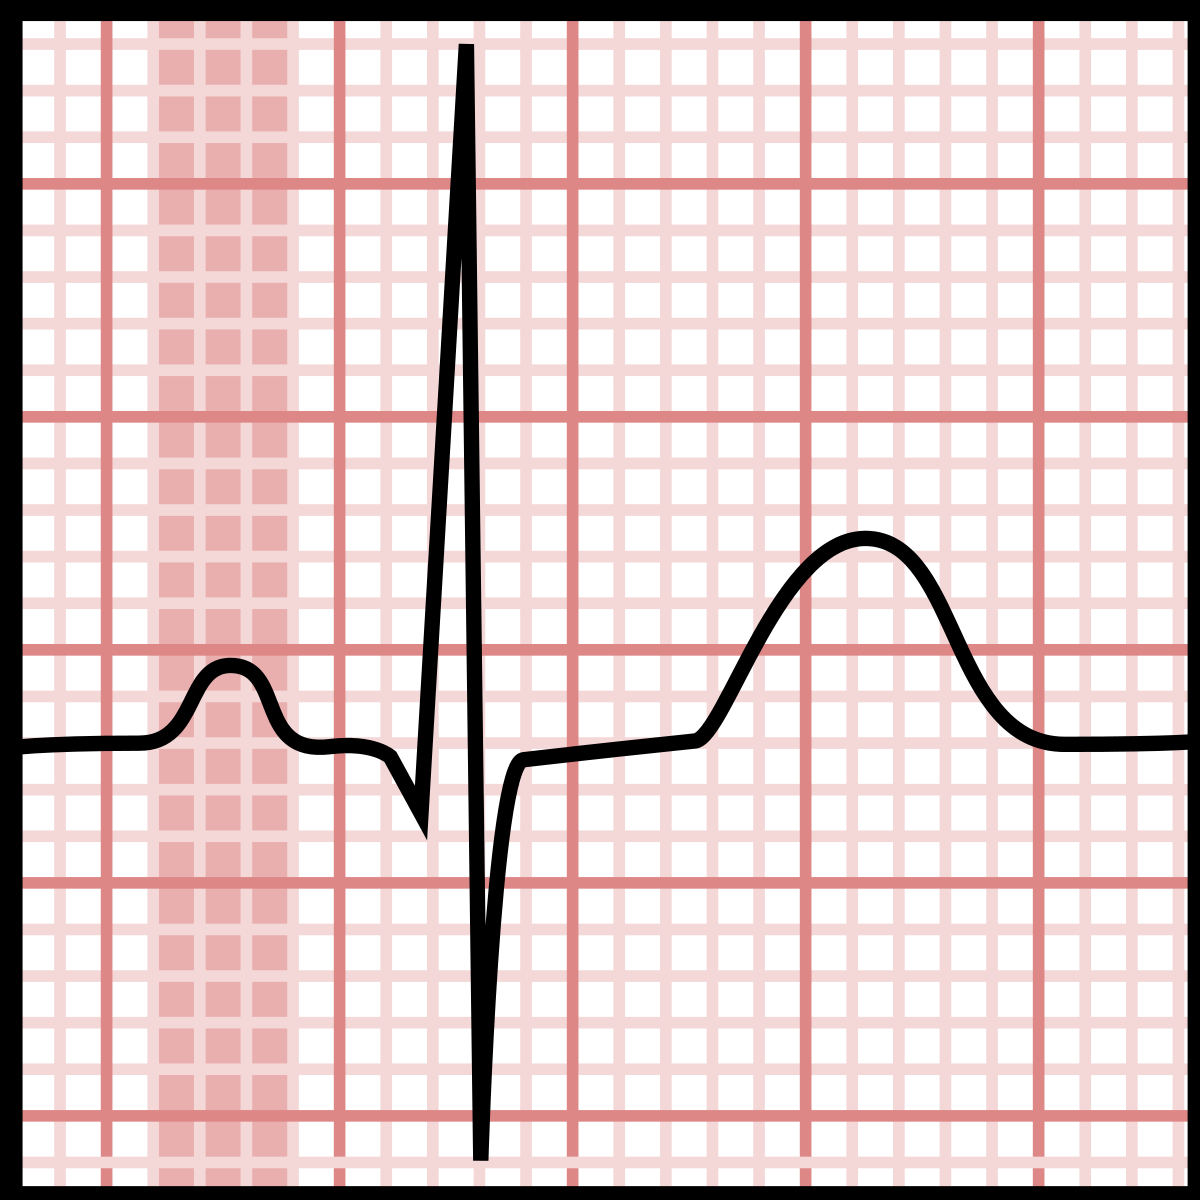
\includegraphics[scale=0.1]{latex_code/Figures_new/p_wave.png}
    \caption{Ρ-κυμάτωση}
    \label{fig:p_wave}
\end{figure}

\begin{figure}[h]
    \centering
    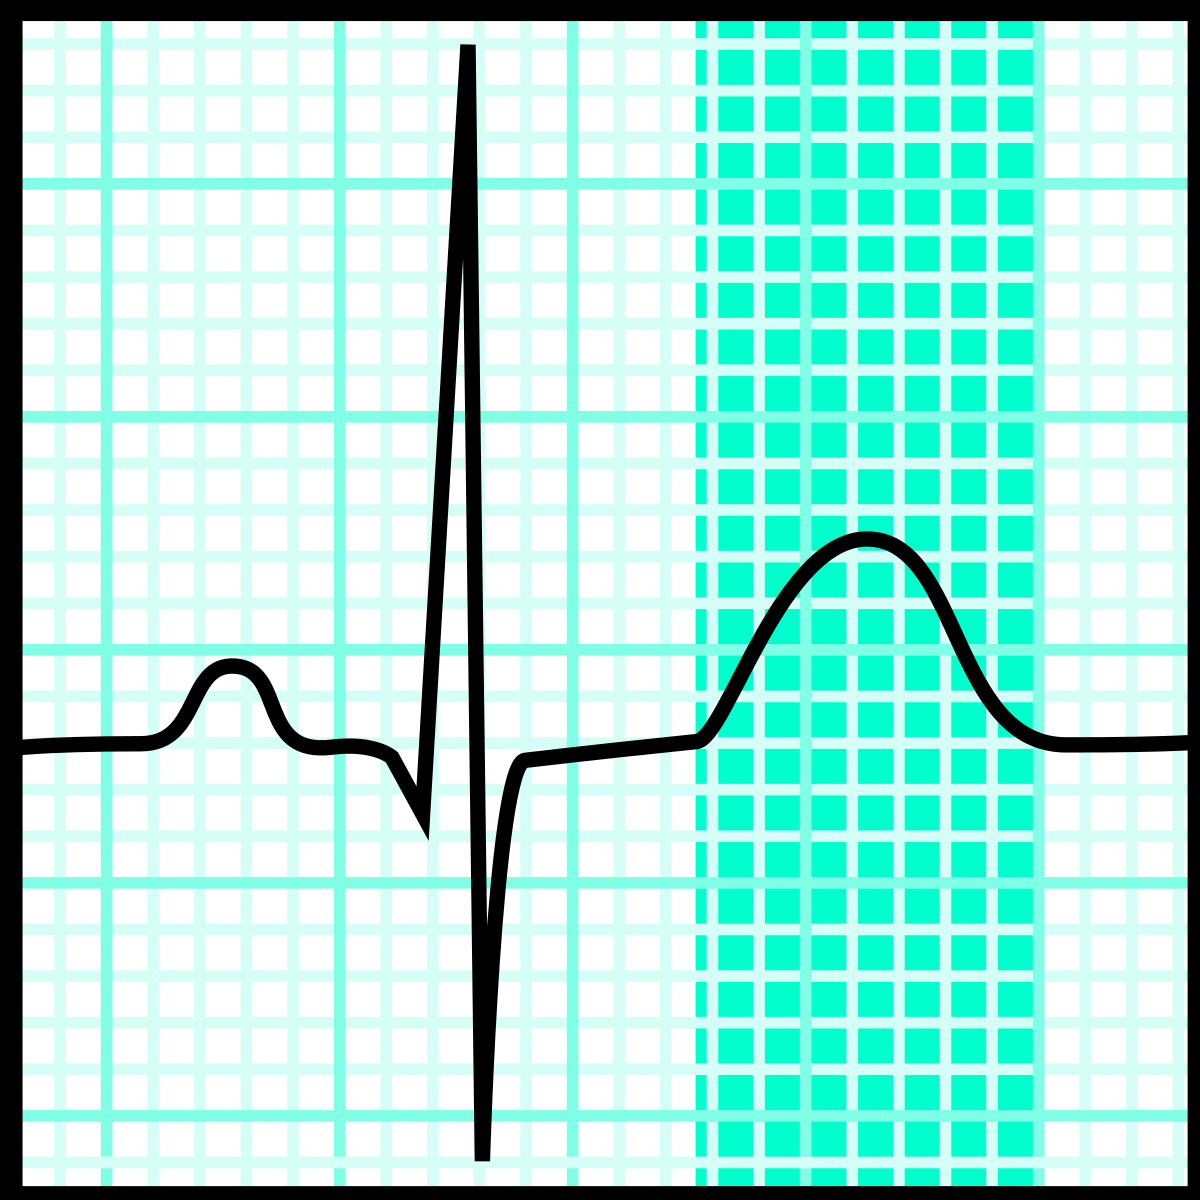
\includegraphics[scale=0.1]{latex_code/Figures_new/t_wave.png}
    \caption{Τ-κυμάτωση}
    \label{fig:t_wave}
\end{figure}

Τα δύο παραπάνω διαστήματα, μας ενδιαφέρουν ιδιαιτέρως, αφενός γιατί η μορφή τους μπορεί να μας δώσει αρκετά χρήσιμα στοιχεία για την αξιολόγηση της φυσιολογικότητας ενός καρδιακού χτύπου, αφετέρου γιατί ενίοτε δημιουργούν προβλήματα στους αλγορίθμους αναγνώρισης των \selectlanguage{english}R\selectlanguage{greek} κορυφών, και συνεπώς χρήζουν ιδιαίτερης σημασίας.

Ανάμεσα στους πολλούς διαθέσιμους αλγόριθμους για τον εντοπισμό των \selectlanguage{english}R\selectlanguage{greek} κορυφών, αποφασίσαμε να χρησιμοποιήσουμε τον αλγόριθμο των \selectlanguage{english}Pan\selectlanguage{greek} και \selectlanguage{english}Tompkins\selectlanguage{greek},\cite{pan_tompkins}, καθώς είναι ένας αλγόριθμος πραγματικού χρόνου, με πολύ καλά αποτελέσματα, μικρές προγραμματιστικές απαιτήσεις και έχει χρησιμοποιηθεί σε πολλές εφαρμογές. Ο αλγόριθμος αυτός δεν χρησιμοποιήθηκε αυτούσιος, αλλά προσαρμόστηκε στα δεδομένα της εφαρμογής.

Στη συνέχεια θα περιγράψουμε τον τρόπο με τον οποίο λειτουργεί ο αλγόριθμος αυτός.


\begin{figure}[h]
    \centering
    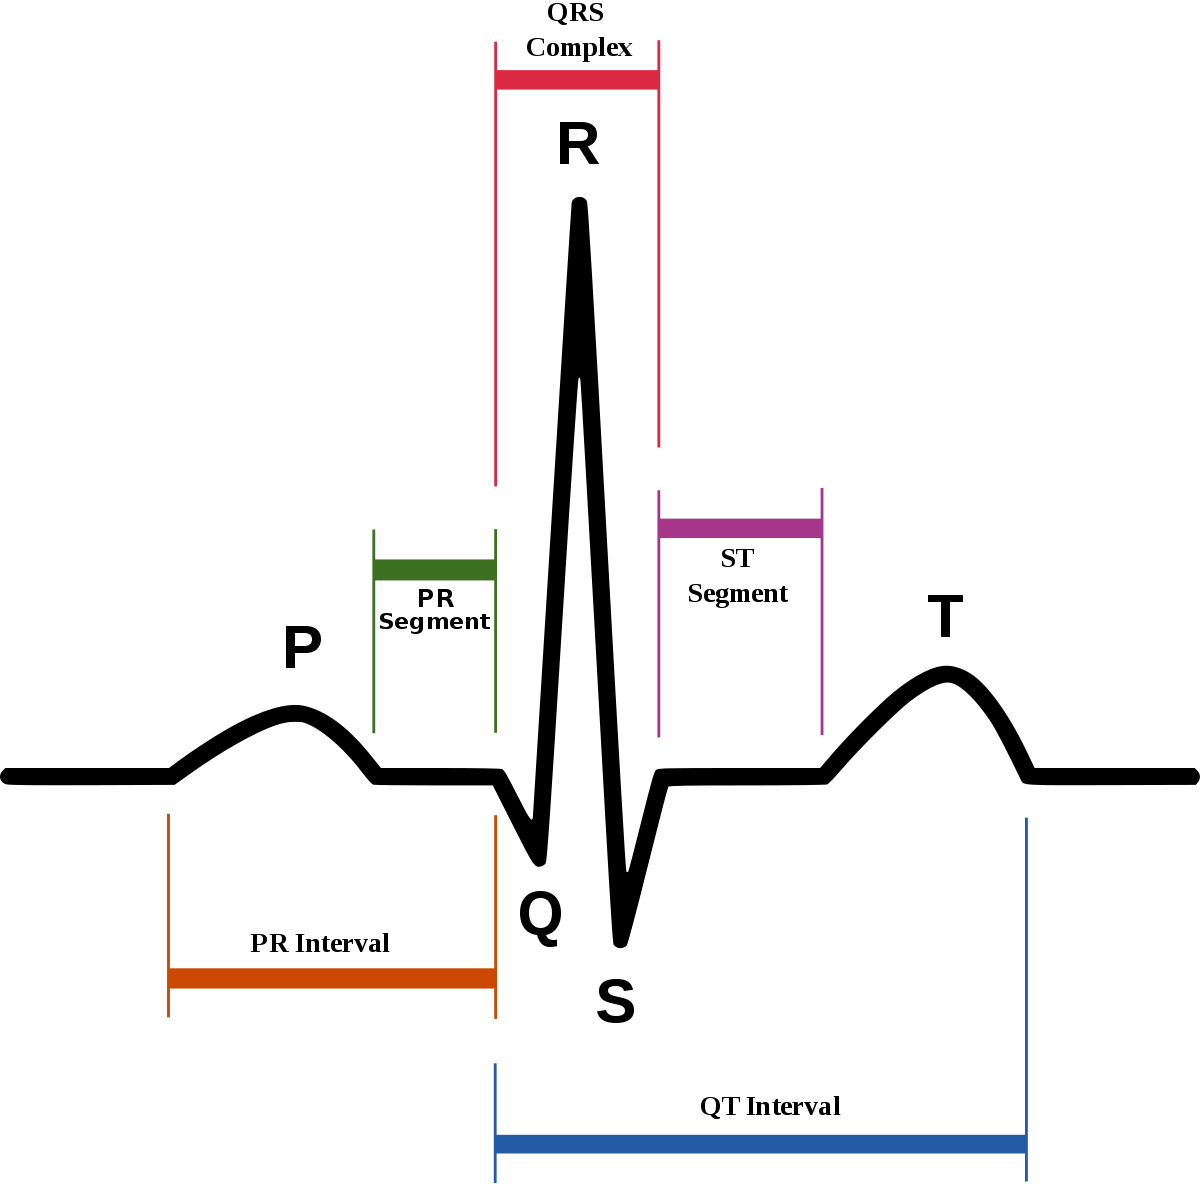
\includegraphics[scale=0.15]{latex_code/Figures_new/qrs.png}
    \caption{Τυπικός διαχωρισμός καρδιακού παλμού σε τμήματα}
    \label{fig:qrs}
\end{figure}

\subsection*{Αλγόριθμος \selectlanguage{english}Pan Tompkins}

\selectlanguage{greek}

\subsubsection*{Εισαγωγικά για τον αλγόριθμο}

Όπως αναφέρθηκε προηγουμένως, ο αλγόριθμος \selectlanguage{english}Pan Tompkins\selectlanguage{greek} είναι ένας αλγόριθμος εντοπισμού κορυφών σε ένα καρδιογράφημα, και είναι πραγματικού χρόνου. Αυτό σημαίνει ότι μπορεί να χρησιμοποιηθεί σε αντίστοιχες εφαρμογές και να δίνει αποτελέσματα την ίδια στιγμή που συμβαίνουν. Ωστόσο, για το πρόβλημα που προσπαθούμε να επιλύσουμε, αυτή η ιδιότητα δεν είναι χρήσιμη, οπότε θα χρησιμοποιήσουμε μια εκδοχή του αλγορίθμου που δεν είναι πραγματικού χρόνου.

Η ανάλυση πραγματικού χρόνου, εισάγει ορισμένους περιορισμούς. Ο πιο σημαντικός εξ αυτών είναι ότι έχουμε να αντιμετωπίσουμε αυστηρά ένα αιτιατό σύστημα. Αντιθέτως, με μια ανάλυση μη πραγματικού χρόνου, μπορούμε να χρησιμοποιήσουμε μη αιτιατά συστήματα, κάτι το οποίο μας επιτρέπει να χρησιμοποιήσουμε "μελοντικές" τιμές μιας κυματομορφής και να εξάγουμε από αυτές χρήσιμη πληροφορία για το "παρόν".

Ένα σημαντικό πλεονέκτημα της παραπάνω ιδιότητας είναι ότι μπορούμε να εφαρμόζουμε ψηφιακά φίλτρα που να εισάγουν μηδενική φάση. Σε αντίθεση με τα \selectlanguage{english}FIR\selectlanguage{greek} φίλτρα \cite{wikiFIR}, που γνωρίζουμε ότι εισάγουν γραμμική φάση αν οι συντελεστές τους είναι συμμετρικοί ως προς το κέντρο τους, τα φίλτρα μηδενικής φάσης δεν εισάγουν καμία φάση, και έτσι μπορούμε να έχουμε το τελικό αποτέλεσμα χωρίς την εισαγωγή καθυστέρησης.

Ο τρόπος με τον οποίο λειτουργούν τα συγκεκριμένα φίλτρα φαίνεται παρακάτω:

\begin{figure}[h]
    \centering
    
\usetikzlibrary{shapes, arrows, positioning}

\selectlanguage{english}

\tikzstyle{block} = [draw, rectangle,
    minimum height=3em, minimum width=4em, align=center, rounded corners = 3pt]
\tikzstyle{sum} = [draw, fill=blue!20, circle, node distance=1cm]
\tikzstyle{input} = [coordinate]
\tikzstyle{output} = [coordinate]
\tikzstyle{pinstyle} = [pin edge={to-,thin,black}]

% The block diagram code is probably more verbose than necessary
\begin{tikzpicture}[auto]
    % We start by placing the blocks
    \node [input, name=input] {};
    % \node [sum, right of=input] (sum) {};
    \node [block] (band) [right=1.5cm of input] {Filter \\ $H(e^{j\omega})$};
    \node [block] (derivative) [right=1.5 cm of band] {Time \\ reverse};
    \node [block] (squaring) [right=1.5cm of derivative] {Filter \\ $H(e^{j\omega})$};
    \node [block] (moving) [right=1.5cm of squaring] {Time \\ reverse};
    \node [output] (output) [right=1.5cm of moving] {};
    % \node [block, right=of controller, pin={[pinstyle]above:Disturbances},
    %         node distance=3cm] (system) {System of Dawn is the system};
    % We draw an edge between the controller and system block to 
    % calculate the coordinate u. We need it to place the measurement block. 
    % \draw [->] (controller) -- node[name=u] {$u$} (system);
    

    % Once the nodes are placed, connecting them is easy. 
    \draw [draw,->] (input) -- node {$x[n]$} (band);
    \draw [->] (band) -- node {$z[n]$} (derivative);
    \draw [->] (derivative) -- node {$w[n]$} (squaring);
    \draw [->] (squaring) -- node {$v[n]$} (moving);
    \draw [->] (moving) -- node [name=y] {$y[n]$}(output);
    % \draw [->] (moving) |- node {} (derivative);
    % \draw [->] (sum) -- node {$e$} (controller);
    % \draw [->] (moving) -- node [name=y]; {$y$}(output);
    % \draw [->] (y) |- (measurements);
    % \draw [->] (measurements) -| node[pos=0.99] {$-$} 
    %     node [near end] {$y_m$} (sum);
\end{tikzpicture}

\selectlanguage{greek}
    \caption{Διάγραμμα φίλτρων μηδενικής φάσης}
    \selectlanguage{greek}
    \label{fig:zero_phase_fir}
\end{figure}

όπου $z[n] = x[n]*h[n]$, $w[n] = z[-n]$, $v[n] = w[n]*h[n]$ και $y[n] = v[-n]$.
Στο πεδίο της συχνότητας, εύκολα υπολογίζουμε από τα παραπάνω την εξής σχέση:
\begin{equation}
\label{eq:zero_phase_eq}
   Y(e^{j\omega}) = |H(e^{j\omega})|^2X(e^{j\omega})
\end{equation}
Όπως βλέπουμε, η τελική συνάρτηση μεταφοράς έχει θετικούς και πραγματικούς συντελεστές, οπότε επιβεβαιώνεται ότι το παραπάνω φίλτρο εισάγει μηδενική φάση.


\begin{figure}[h]
    \centering
    \selectlanguage{english}

\tikzstyle{block} = [draw, rectangle,
    minimum height=3em, minimum width=4em, align=center, rounded corners = 3pt]
\tikzstyle{sum} = [draw, fill=blue!20, circle, node distance=1cm]
\tikzstyle{input} = [coordinate]
\tikzstyle{output} = [coordinate]
\tikzstyle{pinstyle} = [pin edge={to-,thin,black}]

% The block diagram code is probably more verbose than necessary
\begin{tikzpicture}[auto]
    % We start by placing the blocks
    \node [input, name=input1] {};
    % \node [sum, right of=input] (sum) {};
    \node [block]  (band1) [right=1cm of input1] {Band-pass \\ filtering};
    \node [block] (derivative1) [right=1cm of band1] {Derivative filter};
    \node [block] (squaring1) [right=1cm of derivative1] {Squaring};
    \node [block] (moving1) [right=1cm of squaring1] {Moving window \\integration};
    % \node [block, right=of controller, pin={[pinstyle]above:Disturbances},
    %         node distance=3cm] (system) {System of Dawn is the system};
    % We draw an edge between the controller and system block to 
    % calculate the coordinate u. We need it to place the measurement block. 
    % \draw [->] (controller) -- node[name=u] {$u$} (system);
    \node [output1] [right=1cm of moving1] (output1) {};

    % Once the nodes are placed, connecting them is easy. 
    \draw [draw,->] (input1) -- node {$ECG$} (band1);
    \draw [->] (band1) -- node {} (derivative1);
    \draw [->] (derivative1) -- node {} (squaring1);
    \draw [->] (squaring1) -- node {} (moving1);
    % \draw [->] (moving) -- node [name=y] {$y$}(output);
    % \draw [->] (moving) |- node {} (derivative);
    % \draw [->] (sum) -- node {$e$} (controller);
    % \draw [->] (moving) -- node [name=y]; {$y$}(output);
    % \draw [->] (y) |- (measurements);
    % \draw [->] (measurements) -| node[pos=0.99] {$-$} 
    %     node [near end] {$y_m$} (sum);
\end{tikzpicture}

\selectlanguage{greek}
    \caption{Διάγραμμα των σταδίων προεπεξεργασίας του αλγορίθμου}
    \selectlanguage{greek}
    \label{fig:panTompkins_block}
\end{figure}

\subsubsection*{Ακύρωση θορύβου}
Στο πρώτο βήμα του αλγορίθμου εφαρμόζεται ένα ζωνοπερατό φίλτρο \selectlanguage{english}Butterworth\selectlanguage{greek} \cite{wikiButter} τρίτης τάξης, με συχνότητες αποκοπής τα 5 και 15 \selectlanguage{english}Hz\selectlanguage{greek}. Με την εφαρμογή αυτού του φίλτρου, επιχειρείται να αυξηθεί ο λόγος \selectlanguage{english}SNR\selectlanguage{greek}, καθώς έτσι ελαχιστοποιείται ο μυϊκός θόρυβος, οι ηλεκτρομαγνητικές παρεμβολές στο όργανο μέτρησης, αλλά και οι χαμηλής συχνότητας κυματώσεις.

Για τη συχνότητα δειγματοληψίας καρδιογραφήματος του \selectlanguage{english}Apple Watch\selectlanguage{greek} που είναι ίση με 512.414 \selectlanguage{english}Hz\selectlanguage{greek}, το φίλτρο που προκύπτει είναι το εξής:
\begin{equation}
\label{eq:current_butterworth}
   H_1(z) = 0.0002046\frac{1 -3z^{-2}+3z^{-4}-z^{-6}}{1 - 5.723z^{-1} + 13.680z^{-2}-17.485z^{-3}+12.604z^{-4}-4.859z^{-5}+0.782z^{-6}}
\end{equation}

Σημειώνεται ότι η προγραμματιστική υλοποίηση υπολογίζει αυτόματα τους συντελεστές του φίλτρου 
\selectlanguage{english}Butterworth\selectlanguage{greek} αναλόγως τη συχνότητα. Κατόπιν της εφαρμογής του φίλτρου, η νέα κυματομορφή κανονικοποιείται ως προς τη μέγιστη τιμή που εμφανίζεται σε αυτή. Τα αποτελέσματα του αλγορίθμου εμφανίζονται γραφικά στο σχήμα \ref{fig:pan_tompkins_graph}.

\begin{figure}[h]
    \centering
    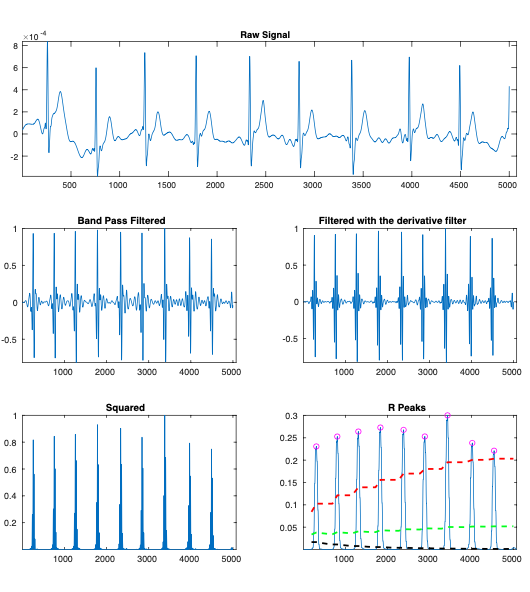
\includegraphics[scale=0.7]{latex_code/Figures_new/graph.png}
    \caption{Στάδια υλοποίησης αλγορίθμου \selectlanguage{english}Pan Tompkins}\selectlanguage{greek}
    \label{fig:pan_tompkins_graph}
\end{figure}

\subsubsection*{Διαφόριση}

Στο δεύτερο στάδιο του αλγορίθμου, εφαρμόζουμε ένα φίλτρο διαφόρισης, έτφσι ώστε να εμφανίζονται πιο έντονες οι γρήγορες εναλλαγές στο σήμα μας. Η αρχική υλοποίηση των \selectlanguage{english}Pan Tompkins\selectlanguage{greek}, για συχνότητα δειγματοληψίας 200 \selectlanguage{english}Hz\selectlanguage{greek}, προτείνει ως φίλτρο διαφόρισης το φίλτρο $H(z) = 0.1(-2z^{-2} - z^{-1} + z^1 +2z^2)$. Στο φίλτρο αυτό όπως βλέπουμε εμφανίζονται δύο διαφορές, η $(z^1-z^{-1})$ και η $2(z^2 - z^{-2})$. 

Αντί αυτού, εμείς θα χρησιμοποιήσουμε την προσαρμοσμένη έκδοση του φίλτρου από τον \selectlanguage{english}Hooman Sedghamiz\selectlanguage{greek} \cite{pan_tompkins_matlab}. Εδώ, το αρχικό φίλτρο που χρησιμοποιείται είναι το φίλτρο $H(z) = (-z^{-3} - 2z^{-2} + 2z^{-1} + 1)$, όπου βλέπουμε πως η μόνη ουσιαστική αλλαγή είναι ότι εναλλάχθηκαν οι συντελεστές των προηγούμενων διαφορών (και μετατοπίστηκαν στο χρόνο ώστε να μπορεί να υλοποιηθεί το φίλτρο χωρίς περαιτέρω επεξεργασία σε υπολογιστή). Συνεπώς, σε μορφή πίνακα, το φίλτρο μας μπορεί να παρασταθεί ως $A = [1, 2, 0, -2, -1]$. (Οι συντελεστές του πίνακα έχουν φθίνοντα αριθμό τάξης)

Χρησιμοποιώντας τον παραπάνω πίνακα, δημιουργούμε έναν καινούργιο πίνακα (και άρα ένα νέο φίλτρο), εφαρμόζοντας γραμμική παρεμβολή στα στοιχεία του πίνακα. Συγκεκριμένα, ξεικνάμε από το πρώτο στοιχείο, και προχωρώντας με βήμα $c = \frac{160}{F_s}$, όπου $F_s$ η συχνότητα δειγματοληψίας, φτάνουμε μέχρι το τελευταίο στοιχείο (χωρίς ωστόσο να το ξεπεράσουμε). Έτσι, ο νέος πίνακας που προκύπτει είναι ο B = [64.1, 84.1, 104.1, 124.1, 96.2, 56.2, 16.2, -23.8, -63.8, -103.8, -120.3, -100.3, -80.3], και το νέο φίλτρο που προκύπτει είναι το 
\begin{equation}
\label{eq:derivation}
   H_2(z) =  \sum_{n=0}^{12}B(n)\cdot z^{-n}
\end{equation}
Μετά από την εφαρμογή της διαφόρισης, το νέο σήμα κανονικοποιείται με τρόπο παρόμοιο με το προηγούμενο βήμα.

\subsubsection*{Ύψωση στο τετράγωνο}

Στο επόμενο βήμα, υψώνουμε το φιλτραρισμένο σήμα στο τετράγωνο. Η ενέργεια αυτή γίνεται για να τονισθούν ακόμη περισσότερο οι κυρίαρχες κορυφές του σήματος, καθώς επίσης και για να μειωθεί η πιθανότητα να αξιολογήσουμε λανθασμένα μια Τ-κυμάτωση ως κορυφή.

\subsubsection*{Ολοκλήρωση - κινούμενος μέσος}

Στο τελευταίο βήμα προεπεξεργασίας του σήματος εφαρμόζουμε μία ολοκλήρωση, ή ένα φίλτρο κινούμενου μέσου στο σήμα μας. Αυτό υλοποιείται με τη συνέλιξη του επεξεργασμένου σήματός μας με ένα σήμα που αποτελείται από μονάδες, και το μήκος του οποίου (μήκος παραθύρου) είναι ίσο με 150 \selectlanguage{english}msec\selectlanguage{greek}, ή $F_s\cdot0.15$ δείγματα. Μέσω αυτής της διαδικασίας, το σήμα μας αποκτά τη μορφή του 5ου διαγράμματος του σχήματος \ref{fig:pan_tompkins_graph}, στο οποίο φαίνεται ότι τα πολλά συμπιεσμένα ακρότατα που υπήρχαν προηγουμένως κοντά στις \selectlanguage{english}R\selectlanguage{greek} κορυφές έχουν αντικατασταθεί πλέον από μία μόνο κορυφή. Η μορφή αυτή του σήματός μας είναι πλεόν κατάλληλη για να εισαχθεί στον τελικό αλγόριθμο εντοπισμού των \selectlanguage{english}R\selectlanguage{greek} κορυφών.

\subsubsection*{Εντοπισμός μεγίστων}

Χρησιμοποιώντας το φιλτραρισμένο σήμα που έχει προκύψει από τα προηγούμενα στάδια επεξεργασίας, εντοπίζουμε όλα τα τοπικά μέγιστα που υπάρχουν στο σήμα μας. Ως τοπικό μέγιστο θεωρούμε κάθε τιμή της κυματομορφής για την οποία το εξεταζόμενο δείγμα είναι μεγαλύτερο από το προηγούμενο και το επόμενο δείγμα. 

Οι \selectlanguage{english}R\selectlanguage{greek} κορυφές του σήματός μας υπάγονται σε έναν σημαντικό περιορισμό εξαιτίας της φυσιολογίας της καρδιάς. Συγκεκριμένα, δεν μπορούν να απέχουν μεταξύ τους λιγότερο από 200 \selectlanguage{english}msec\selectlanguage{greek}, καθώς αυτή είναι η ελάχιστη περίοδος ανάκαμψης της καρδιάς (Τ-κυμάτωση) \cite{wikiT_wave}. 

Συνεπώς, ελέγχουμε τα μέγιστα σημεία που έχουμε βρει, και από όσα απέχουν μεταξύ τους λιγότερο από 200 \selectlanguage{english}msec\selectlanguage{greek} κρατάμε μόνο αυτά που έχουν την υψηλότερη τιμή (δηλαδή αυτά που έχουν τη μεγαλύτερη πιθανότητα να είναι όντως \selectlanguage{english}R\selectlanguage{greek} κορυφές).

\subsubsection*{Κατώφλια}

Κάθε ένα από τα ακρότατα που έχουμε βρει στο προηγούμενο βήμα θεωρείται υποψήφια κορυφή. Για να μειώσουμε την πιθανότητα να επιλέξουμε λανθασμένα ένα σημείο ως κορυφή, συγκρίνουμε όλα τα σημεία με ένα υπάρχον κατώφλι $(Threshold1)$, το οποίο έχει διαμορφωθεί από τις προηγούμενες κορυφές που βρήκαμε, λαμβάνοντας υπόψιν τα επίπεδα θορύβου στο σήμα, με βάση τον παρακάτω τύπο:

\begin{equation}
\label{eq:threshold1}
   Threshold_1 = NoiseLevel_1 + 0.25(SignalLevel_1 - NoiseLevel_1)
\end{equation}

όπου $NoiseLevel_1$ είναι η τρέχουσα εκτίμηση του επιπέδου του θορύβου (δηλαδή των ψευδών κορυφών) και $SignalLevel_1$ η τρέχουσα εκτίμηση του επιπέδου του σήματος (δηλαδή του επιπέδου στο οποίο βρίσκονται οι πραγματικές κορυφές) στο σήμα που έχει προκύψει μετά την εφαρμογή του κινούμενου μέσου.

Οι παραπάνω όροι, και κατ' επέκταση το κατώφλι, ανανεώνονται αυτόματα μετά από την ταξινόμηση μιας κορυφής ως πραγματική κορυφή ή ως ψευδή κορυφή (θόρυβος) ως εξής:

Εάν η κορυφή $PEAK_I$ είναι πραγματική κορυφή:
\begin{equation}
\label{eq:threshold1_renewal}
   SignalLevel_I = 0.125PEAK_I + 0.875SignalLevel_I 
\end{equation}

Εάν η κορυφή $PEAK_I$ είναι κορυφή θορύβου:
\begin{equation}
\label{eq:threshold1_renewal}
   NoiseLevel_I = 0.125PEAK_I + 0.875NoiseLevel_I 
\end{equation}

όπου $PEAK_I$ είναι η νέα υποψήφια κορυφή που εντοπίστηκε.

Στην αρχή του αλγορίθμου, χρειάζεται ένα διάστημα 2 δευτερολέπτων για να αρχικοποιηθούν τα παραπάνω κατώφλια. Η αρχικοποίηση γίνεται με βάση τις παρακάτω σχέσεις:

\begin{equation}
\label{eq:threshold1_starting_conditions}
\begin{array}{l}
    & Threshold_1 = 1/3\cdot max\{ECG_M\}
    & SignalLevel_1 = Threshold_1
    & NoiseLevel_1 = 1/2 \cdot E(ECG_M)
\end{array}
\end{equation}

όπου $max\{ECG_M\}$ η μέγιστη τιμή της κυματομορφής μετά την εφαρμογή κινούμενου μέσου για τα δύο πρώτα δευτερόλεπτα, και $E(ECG_M)$ η μέση τιμή της ίδιας κυματομορφής για τα δύο πρώτα δευτερόλεπτα.

Εάν η τιμή της κορυφής $PEAK_I$ είναι μικρότερη από το κατώφλι $Threshold_1$, τότε αξιολογείται ως κορυφή θορύβου. Εάν είναι μεγαλύτερη από το $Threshold_1$, τότε γίνεται ένας περαιτέρω έλεγχος για να αξιολογηθεί ως \selectlanguage{english}R\selectlanguage{greek}.

Αρχικά βρίσκουμε το αντίστοιχο σημείο στο σήμα που έχει υποστεί μόνο το ζωνοπερατό φίλτρο. Κατ' αντιστοιχία με τα προηγούμενα κατώφλια που ορίστηκαν, ορίζουμε τα νέα κατώφλια:
\begin{equation}
\label{eq:thresholdf}
\begin{array}{l}
    & Threshold_F = NoiseLevel_F + 0.25(SignalLevel_F - NoiseLevel_F)
\end{array}
\end{equation}

Εάν η κορυφή $PEAK_F$ είναι πραγματική κορυφή:
\begin{equation}
\label{eq:thresholdf_renewal}
   SignalLevel_F = 0.125PEAK_F + 0.875SignalLevel_F 
\end{equation}

Εάν η κορυφή $PEAK_F$ είναι κορυφή θορύβου:
\begin{equation}
\label{eq:thresholdf_renewal}
   NoiseLevel_F = 0.125PEAK_F + 0.875NoiseLevel_F 
\end{equation}

Οι αρχικές συνθήκες των κατωφλιών αυτών ορίζονται κατ' αναλογία ως εξής:

\begin{equation}
\label{eq:thresholdf_starting_conditions}
\begin{array}{l}
    & Threshold_F = 1/3\cdot max\{ECG_B\}
    & SignalLevel_F = Threshold_F
    & NoiseLevel_F = 1/2 \cdot E(ECG_F)
\end{array}
\end{equation}

όπου $max\{ECG_B\}$ η μέγιστη τιμή της κυματομορφής μετά την εφαρμογή του ζωνοπερατού φίλτρου για τα δύο πρώτα δευτερόλεπτα, και $E(ECG_B)$ η μέση τιμή της ίδιας κυματομορφής για τα δύο πρώτα δευτερόλεπτα. Εάν η κορυφή είναι μεγαλύτερη από το κατώφλι $Threshold_F$, τότε κατατάσσεται τελικά ως πραγματική κορυφή και ανανεώνεται το κατώλφι $SignalLevel_F$. Διαφορετικά, κατατάσσεται ως κορυφή θορύβου και ανανεώνεται το κατώφλι $NoiseLevel_F$.

Μια περαιτέρω δικλίδα ασφαλείας για τη σωστή αξιολόγηση των κατωφλιών $Threshold_I$ και $Threshold_F$ λαμβάνει υπόψη τα διαστήματα που μεσολαβούν μεταξύ των φερόμενων \selectlanguage{english}R\selectlanguage{greek} κορυφών. Συγκεκριμένα, ελέγχεται συνεχώς η μέση χρονική απόσταση μεταξύ των χτύπων, για τα τελευταία 8 ζευγάρια χτύπων. Εάν η νέα χρονική απόσταση που σημειώνεται είναι μεγαλύτερη από το 116\% ή μικρότερη από το 92\% αυτής της τιμής, τότε τα κατώφλια $Threshold_I$ και $Threshold_F$ υποδιπλασιάζονται, γιατί υπάρχει η υποψία ότι ο αλγόριθμος έχει αποκτήσει πλέον πολύ υψηλό κατώφλι.

\subsubsection*{Επανέλεγχος για μη εντοπισμένες κορυφές}

Σε περίπτωση που δεν έχει εμφανιστεί κάποιος χτύπος για ένα διάστημα μεγαλύτερο ή ίσο με το 166\% της μέσης χρονικής διαφοράς μεταξύ δύο χτύπων (υπολογισμένη στα τελευταία 8 ζευγάρια), τότε ο αλγόριθμος εντοπίζει τη μέγιστη τιμή του σήματος που έχει προκύψει από τον κινούμενο μέσο σε αυτό το διάστημα και την αντιμετωπίζει ως πιθανή κορυφή. Τα κατώφλια σύγκρισης που χρησιμοποιούνται είναι υποδιπλασιασμένα σε σχέση με την κανονική τιμή τους.

Ο παραπάνω περιορισμός, προστίθεται εξαιτίας της φυσιολογίας της καρδιάς, που επιβάλλει συγκεκριμένα όρια στη χρονική απόσταση μεταξύ δύο διαδοχικών καρδιακών χτύπων \cite{pan_tompkins}.

\subsubsection*{Έλεγχος λανθασμένου εντοπισμού Τ-κυμάτωσης}

Ο αλγόριθμος δίνει ιδαίτερη έμφαση στην αποφυγή του λανθασμένου χαρακτηρισμού μιας Τ-κυμάτωσης ως \selectlanguage{english}R\selectlanguage{greek} κορυφής. Συγκεκριμένα, σε περίπτωση που ο νέος υποψήφιος χτύπος έχει εμφανιστεί σε μικρότερη απόσταση από 360 \selectlanguage{english}ms\selectlanguage{greek} από τον προηγούμενο χτύπο, υπάρχει σημαντικό ενδεχόμενο να πρόκειται για μια Τ-κυμάτωση. Συνεπώς, ελέγχεται η κλίση του σήματος που έχει προκύψει από το φίλτρο κινούμενου μέσου. 

Συγκεκριμένα χρησιμοποιούμε τη μέση τιμή των διαδοχικών διαφορών του σήματος αυτού για τα τελευταία 75 \selectlanguage{english}ms\selectlanguage{greek} μέχρι το φερόμενο χτύπο. Το μέτρο αυτό εκφράζει ουσιαστικά το μέσο ρυθμό μεταβολής του σήματος. Το χαρακτηριστικό ενός διαστήματος \selectlanguage{english}QRS\selectlanguage{greek} είναι ότι έχει σαφώς γρηγορότερο ρυθμό μεταβολής από ότι μια Τ-κυμάτωση. Αν η τιμή της παραπάνω μετρικής για τον υποψήφιο χτύπο είναι μικρότερη από το μισό της αντίστοιχης μετρικής του προηγούμενου χτύπου, τότε το σημείο που εντοπίσαμε είναι η κορυφή της Τ-κυμάτωσης και συνεπώς αξιολογείται ως θόρυβος. Διαφορετικά, αξιολογείται ως \selectlanguage{english}R\selectlanguage{greek} κορυφή.

\begin{figure}[h]
    \centering
    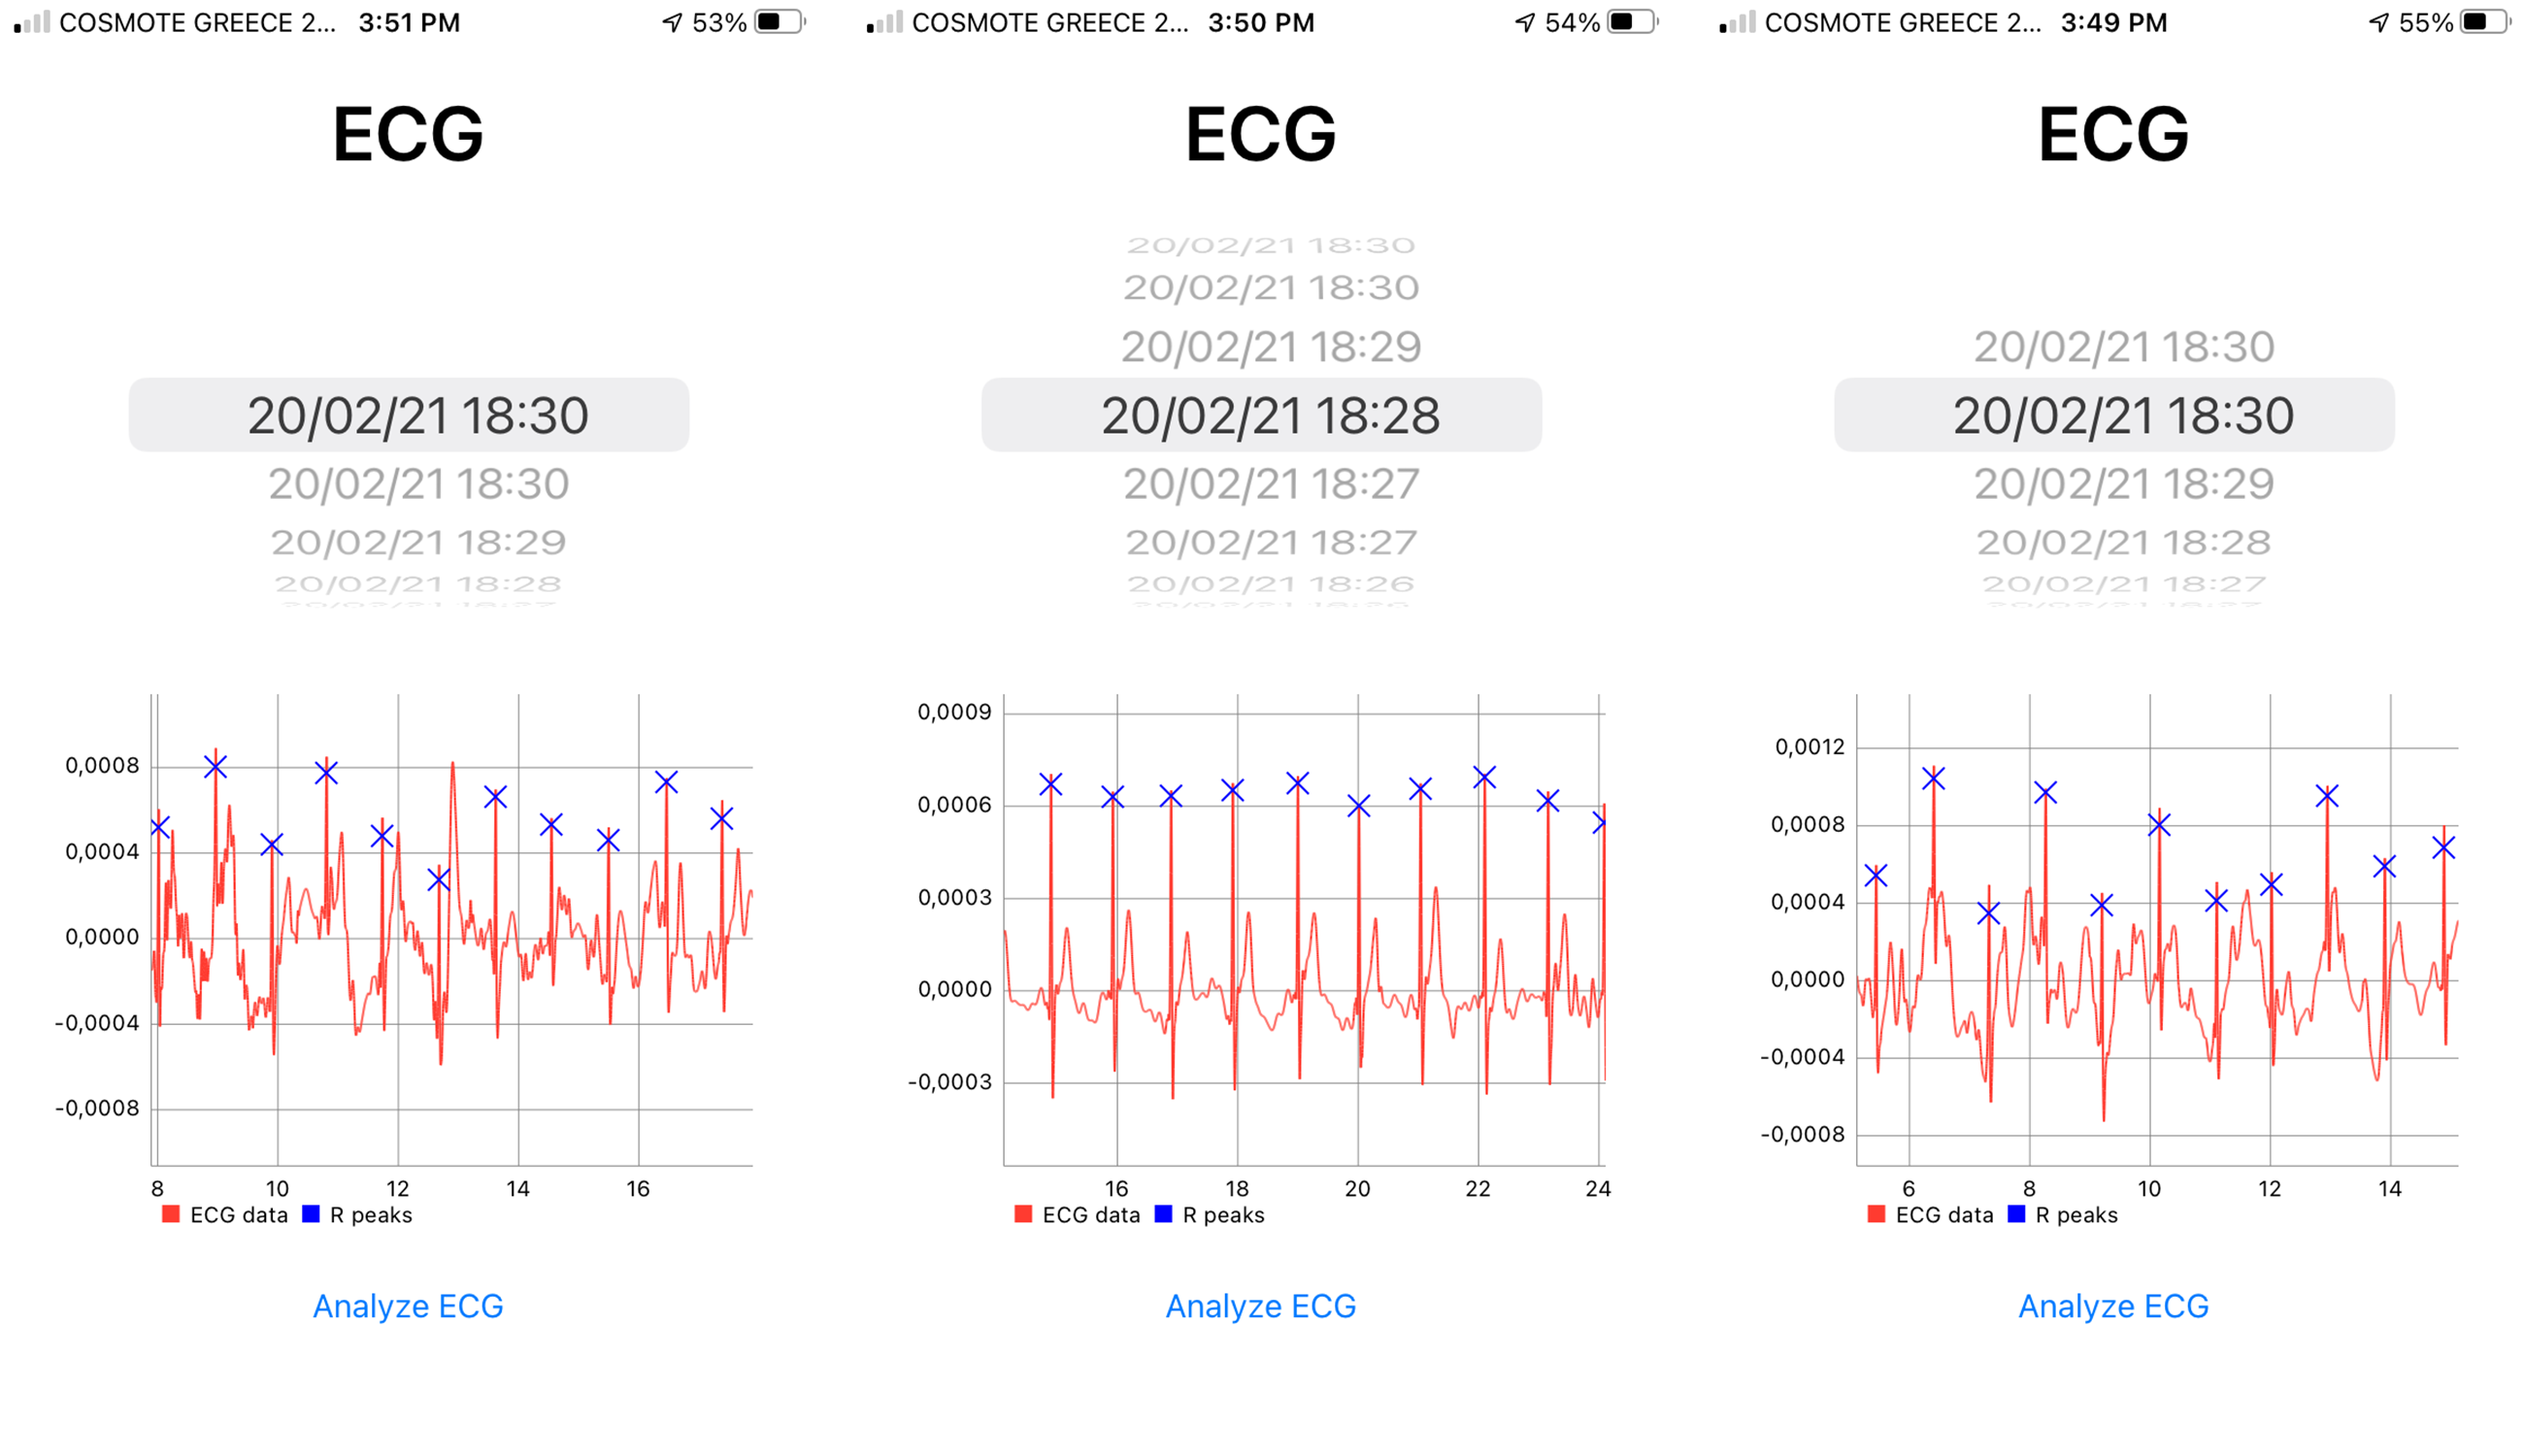
\includegraphics[scale=0.17]{latex_code/Figures_new/ecg_full.png}
    \caption{Αποτέλεσμα εντοπισμού \selectlanguage{english}R\selectlanguage{greek} κορυφών}
    \label{fig:ecg_easy}
\end{figure}


\subsubsection{Αποτελέσματα αλγορίθμου}

Τα αποτελέσματα του αλγορίθμου δεν ελέγχθηκαν εκτενώς, καθώς κάτι τέτοιο έχει γίνει στο παρελθόν από πολλούς ερευνητές \cite{Fariha_2020} \cite{pan_tompkins_matlab}, και στη συντριπτική πλειοψηφία των ελέγχων, ο αλγόριθμος επιτυγχάνει ποσοστά ακρίβειας μεγαλύτερα από 98\%, τα οποία για την παρούσα εφαρμογή είναι ικανοποιητικά. Παρόλα αυτά, ο αλγόριθμος ελέγχθηκε οπτικά σε αρκετά διαθέσιμα καρδιογραφήματα και τα αποτελέσματα ήταν τα αναμενόμενα. Μια οπτική αναπαράσταση των αποτελεσμάτων, φαίνεται στο σχήμα \ref{fig:ecg_easy}.



\subsection{Εξαγωγή χαρακτηριστικών}

Τα χαρακτηριστικά που εξήχθησαν, εννοιολογικά, χωρίζονται στις εξής τρεις κατηγορίες:
\begin{itemize}
    \item Χαρακτηριστικά στο πεδίο του χρόνου
    \item Χαρακτηριστικά στο πεδίο της συχνότητας
    \item Μη γραμμικά χαρακτηριστικά
\end{itemize}

Στη συνέχεια θα αναλύσουμε την κάθε κατηγορία ξεχωριστά και θα παρουσιάσουμε αναλυτικά όλα τα εξαγόμενα χαρακτηριστικά.

\subsubsection*{Ορισμός συνήθων μαθηματικών μεγεθών και στατιστικών μέτρων}
Παρακάτω ορίζονται μερικά συνήθη μαθηματικά μεγέθη και στατιστικά μέτρα που χρησιμοποιήθηκαν στην ανάλυσή μας.
\paragraph{Δειγματική μέση τιμή}
Η δειγματική μέση τιμή ενός μεγέθους \selectlanguage{english}x\selectlanguage{greek} ορίζεται ως εξής:
\begin{equation}
\label{eq:mean}
   \overline{x}=\frac{\sum_{j=1}^{N} x_j}{N}
\end{equation}
όπου \selectlanguage{english}$x_j$\selectlanguage{greek} μια παρατήρηση του μεγέθους, και Ν το πλήθος των παρατηρήσεων. Η δειγματική μέση τιμή, ή απλά μέση τιμή ενός μεγέθους \selectlanguage{english}x\selectlanguage{greek} θα συμβολίζεται ως \selectlanguage{english}$\overline{x}$\selectlanguage{greek}, ή ως $E(x)$.

\paragraph{Τυπική απόκλιση}
Η τυπική απόκλιση ενός μεγέθους \selectlanguage{english}x\selectlanguage{greek} ορίζεται ως εξής:
\begin{equation}
\label{eq:standard_deviation}
   \sigma(x)=\sqrt{\frac{\sum_{j=1}^{N} |x_j-\overline{x}|^2 }{N-1}}
\end{equation}
όπου \selectlanguage{english}$x_j$\selectlanguage{greek} μια παρατήρηση του μεγέθους, και Ν το πλήθος των παρατηρήσεων. Η τυπική απόκλιση ενός μεγέθους \selectlanguage{english}x\selectlanguage{greek} θα συμβολίζεται ως \selectlanguage{english}$\sigma(x)$\selectlanguage{greek}.


\paragraph{\selectlanguage{english}R-R\selectlanguage{greek} διάστημα}
Ως \selectlanguage{english}R-R\selectlanguage{greek} διάστημα, ορίζουμε τη χρονική διαφορά
\begin{equation}
\label{eq:RR}
   RR_i = t(R_{i+1}) - t(R_i)
\end{equation}
όπου \selectlanguage{english}$t(R_i)$\selectlanguage{greek} η χρονική στιγμή που συμβαίνει ο χτύπος (\selectlanguage{english}R\selectlanguage{greek} σημείο) \selectlanguage{english}i\selectlanguage{greek}. Το \selectlanguage{english}R-R\selectlanguage{greek} διάστημα, που ουσιαστικά μετράει τη διάρκεια μεταξύ δύο διαδοχικών καρδιακών χτύπων, θα μετριέται κατά σύμβαση σε χιλιοστά του δευτερολέπτου, και θα συμβολίζεται ως \selectlanguage{english}$RR_i$\selectlanguage{greek}.


\paragraph{Ν-Ν διάστημα}
Το σύνολο των Ν-Ν διαστημάτων είναι ένα υποσύνολο των \selectlanguage{english}R-R\selectlanguage{greek} διαστημάτων. Τόσο το \selectlanguage{english}R-R\selectlanguage{greek} σύνολο, όσο και το Ν-Ν είναι διατεταγμένα σύνολα, δηλαδή η σειρά με την οποία έρχονται τα στοιχεία τους έχει σημασία. Προγραμματιστικά, υλοποιούνται με τη χρήση μιας απλής λίστας, ή ενός μονοδιάστατου πίνακα. Το σύνολο Ν-Ν δημιουργείται από τον εξής αλγόριθμο:
\begin{enumerate}
    \item Αρχικά το σύνολο Ν-Ν είναι ένα κενό σύνολο.
    \item Δημιουργείται μια κενή "ουρά" τεσσάρων θέσεων, την οποία θα ονομάζουμε ουρά σύγκρισης (ΟΣ). Με τον όρο "ουρά", εννοούμε μια δομή δεδομένων \selectlanguage{english}First In First Out\selectlanguage{greek}. Η μέση τιμή των στοιχείων της ουράς συμβολίζεται ως $\overline{O\Sigma}$.
    \item Η ΟΣ γεμίζει για πρώτη φορά, με τρόπο που θα αναλύσουμε πιο κάτω από τον βασικό αλγόριθμο, για λόγους ευκολίας ανάγνωσης.
    \item Για κάθε στοιχείο $RR_i$ του \selectlanguage{english}R-R\selectlanguage{greek} πίνακα κάνουμε τα εξής:
    \begin{enumerate}
        \item Αν $ 0.85 \cdot \overline{O\Sigma} \le RR_i \le 1.15 \cdot \overline{O\Sigma} $, προσθέτουμε την $RR_i$ στο τέλος του πίνακα των Ν-Ν, και εισάγουμε το στοιχείο αυτό στην ΟΣ.
        \item Αλλιώς, εάν $ 0.75 \cdot \overline{O\Sigma} \le RR_i \le 1.25 \cdot \overline{O\Sigma} $, εισάγουμε το στοιχείο στην ΟΣ.
    \end{enumerate}
\end{enumerate}
Για την αρχικοποίηση της ΟΣ, δημιουρηούμε έναν κινούμενο μέσο (ΚΜ) 8 στοιχείων, δηλαδή παίρνουμε την μέση τιμή των 8 πρώτων στοιχείων. Μέχρι να γεμίσει η ΟΣ, ελέγχουμε εάν $ 0.75 \cdot KM \le RR_i \le 1.25 \cdot KM $, και σε περίπτωση που αυτό ισχύει, προσθέτουμε το $RR_i$ στοιχείο στην ΟΣ. Στη συνέχεια, ανανεώνουμε τον ΚΜ ξεκινώντας από το επόμενο στοιχείο και επαναλαμβάνουμε μέχρι να πληροίται η συνθήκη τερματισμού.

Μια ερμηνεία των Ν-Ν διαστημάτων είναι ότι πρόκειται για τα "φυσιολογικά" διαστήματα σε ένα καρδιογράφημα, εννοώντας τα διαστήματα που δεν έχουν πολύ σημαντικές διαφορές στη χρονική τους διάρκεια σε σύγκριση με τα γειτονικά τους. Καθώς οι κορυφές των καρδιακών χτύπων εντοπίζονται αλγοριθμικά, ορισμένες φορές ο αλγόριθμος μπορεί να οδηγήσει σε λανθασμένα αποτελέσματα, που με τη σειρά τους μπορούν να οδηγήσουν σε έντονες μεταβολές στη διάρκεια των \selectlanguage{english}R-R\selectlanguage{greek} διαστημάτων. Χρησιμποιώντας το σύνολο Ν-Ν, το πρόβλημα αυτό περιορίζεται σημαντικά.

Ο παραπάνω αλγόριθμος, διασφαλίζει ένα ποσοστιαίο όριο απόκλισης του κάθε διαστήματος από τα γειτονικά του. Όταν ξεπερνιέται το όριο αυτό, το παρόν διάστημα δεν αξιολογείται ως φυσιολογικό. Πέρα από αυτό όμως, υπάρχει ένα ακόμα όριο, περισσότερο ελαστικό, που καθορίζει εάν το παρόν διάστημα θα χρησιμοποιηθεί ως διάστημα σύγκρισης για τα επόμενα. Ο λόγος που υφίσταται το όριο αυτό και είναι πιο ελαστικό, είναι για να αποφεύγονται καταστάσεις αστάθειας στο σύστημα. Ο αλγόριθμος αυτός είναι μια προσαρμογή του αλγόριθμου των Barbara Mali κ.α. \cite{barbara_mali_alg}

\subsubsection{Χαρακτηριστικά στο πεδίο του χρόνου}

Τα χαρακτηριστικά στο πεδίο του χρόνου ποσοτικοποιούν το μέγεθος της διακύμανσης του καρδιακού ρυθμού, και, ως επί τω πλείστω, είναι στατιστικές μετρικές που σχετίζονται άμεσα με το παρατηρούμενο μέγεθος (ΔΚΡ). Παρακάτω, παρουσιάζονται αναλυτικά.


\paragraph{\selectlanguage{english}SDRR\selectlanguage{greek}}
\selectlanguage{greek}
Η μετρική \selectlanguage{english}SDRR (Standard Deviation of R-R Intervals) \selectlanguage{greek}είναι η τυπική απόκλιση όλων των διαστημάτων  \selectlanguage{english}R-R\selectlanguage{greek}. Δίνεται από τον τύπο
\begin{equation}
\label{eq:SDRR}
   SDRR=\sigma(RR_i)
\end{equation}
Υπολογίζεται σε χιλιοστά του δευτερολέπτου.

\paragraph{\selectlanguage{english}AHR\selectlanguage{greek}}
Η μετρική \selectlanguage{english}AHR (Average Heart Rate) \selectlanguage{greek}εκφράζει τους μέσους χτύπους ανά λεπτό. Δίνεται από τον τύπο
\begin{equation}
\label{eq:AHR}
   AHR=\frac{60}{\overline{RR_i}}
\end{equation}
Υπολογίζεται σε χτύπους ανά λεπτό.

\paragraph{\selectlanguage{english}SDNN\selectlanguage{greek}}
Η μετρική \selectlanguage{english}SDNN (Standard Deviation of N-N Intervals)  \selectlanguage{greek}ποσοτικοποιεί την τυπική απόκλιση των Ν-Ν διαστημάτων. Δίνεται από τον τύπο
\begin{equation}
\label{eq:SDRR}
   SDNN=\sigma(NN_i)
\end{equation}
Υπολογίζεται σε χιλιοστά του δευτερολέπτου.

\paragraph{\selectlanguage{english}SDSD\selectlanguage{greek}}
Η μετρική \selectlanguage{english}SDSD (Standard Deviation of Successive Differences)  \selectlanguage{greek}ποσοτικοποιεί την τυπική απόκλιση μεταξύ των διαφορών των διακρειών δύο γειτονικών Ν-Ν διαστημάτων. Δίνεται από τον τύπο
\begin{equation}
\label{eq:SDRR}
   SDSD=\sigma(|NN_{i+1} - NN_i|)
\end{equation}
Υπολογίζεται σε χιλιοστά του δευτερολέπτου.

\paragraph{\selectlanguage{english}SDANN\selectlanguage{greek}}
Η μετρική \selectlanguage{english}SDANN (Standard Deviation of Average N-N Intervals on Ultra Short Intervals)  \selectlanguage{greek} εκφράζει την τυπική απόκλιση μεταξύ των μέσων τιμών των διαρκειών των Ν-Ν διαστημάτων, σε κάθε υποδιάστημα των 30 δευτερολέπτων του συνολικού δείγματος (διάρκειας 5 λεπτών).

Ουσιαστικά, χωρίζουμε το κάθε δείγμα σε 10 διαστήματα των 30 δευτερολέπτων, υπολογίζουμε τη μέση τιμή διάρκειας του Ν-Ν διαστήματος για κάθε ένα από τα 10 διαστήματα, και τέλος λαμβάνουμε την τυπική απόκλιση αυτών των 10 τιμών. Δίνεται από τον τύπο
\begin{equation}
\label{eq:SDANN}
   SDANN=\sigma(E((NN_i)_{UST}))
\end{equation}

Με τον όρο \selectlanguage{english}"UST"\selectlanguage{greek} εννοούμε το κάθε διάστημα πολύ μικρής διάρκειας. Υπολογίζεται σε χιλιοστά του δευτερολέπτου.

\paragraph{\selectlanguage{english}SDNNI\selectlanguage{greek}}
Η μετρική \selectlanguage{english}SDNNI (Mean of Standard Deviations of N-N Intervals on Ultra Short Intervals)  \selectlanguage{greek} εκφράζει τη μέση τιμή μεταξύ των τυπικών αποκλίσεων των διαρκειών των Ν-Ν διαστημάτων, σε κάθε υποδιάστημα των 30 δευτερολέπτων του συνολικού δείγματος (διάρκειας 5 λεπτών).

Ουσιαστικά, χωρίζουμε το κάθε δείγμα σε 10 διαστήματα των 30 δευτερολέπτων, υπολογίζουμε την τυπική απόκλιση διάρκειας του Ν-Ν διαστήματος για κάθε ένα από τα 10 διαστήματα, και τέλος λαμβάνουμε τη μέση τιμή αυτών των 10 τιμών. Δίνεται από τον τύπο
\begin{equation}
\label{eq:SDNNI}
   SDNNI=E((\sigma(NN_i)_{UST}))
\end{equation}

Με τον όρο \selectlanguage{english}"UST"\selectlanguage{greek} εννοούμε το κάθε διάστημα πολύ μικρής διάρκειας. Υπολογίζεται σε χιλιοστά του δευτερολέπτου.

\paragraph{\selectlanguage{english}pNN50\selectlanguage{greek}}
Η μετρική \selectlanguage{english}pNN50 (Percentage of Adjacent N-N intervals With More Than 50 msec Difference)  \selectlanguage{greek} εκφράζει το ποσοστό των γειτονικών διαστημάτων Ν-Ν που έχουν μεγαλύτερη διαφορά μεταξύ τους από 50 \selectlanguage{english}msec.\selectlanguage{greek}

\paragraph{\selectlanguage{english}RMSSD\selectlanguage{greek}}
Η μετρική \selectlanguage{english}RMSSD (Root Mean Square of Successive Differences)\selectlanguage{greek} δίνεται από τον τύπο 
\begin{equation}
\label{eq:RMSSD}
   RMSSD = \sqrt{\frac{1}{N-1}\cdot\sum_{j=1}^N(NN_j)^2}
\end{equation}
όπου Ν είναι το πλήθος των παρατηρήσεων. Υπολογίζεται σε χιλιοστά του δευτερολέπτου.

\paragraph{\selectlanguage{english}HTI\selectlanguage{greek}}
Η μετρική \selectlanguage{english}HTI (Heart Rate Variability Triangular Index)\selectlanguage{greek} είναι μια γεωμετρική ερμηνεία που προκύπτει από τη ΔΚΡ. Υπολογίζεται ως εξής:
\begin{enumerate}
    \item Δημιουργούμε ένα ιστόγραμμα με τις διάρκειες των Ν-Ν διαστημάτων, και το πλήθος των διαστημάτων που έχουν αυτή τη διάρκεια. Το βήμα, ή η διακριτικότητα των διαστημάτων αυτών είναι ο ακέραιος αριθμός που βρίσκεται πιο κοντά στα 8 χιλιοστά του δευτερολέπτου. Για παράδειγμα, ένα διάστημα με διάρκεια 720 χιλιοστά και συχνότητα δειγματοληψίας 125 \selectlanguage{english}Hz\selectlanguage{greek} θα έχει διακριτική ικανότητα ένα δείγμα, και άρα το παραπάνω διάστημα θα εισαχθεί στο ιστόγραμμα με την τιμή 90.
    \item Μόλις ολοκληρωθεί η παραπάνω διαδικασία, βρίσκουμε την μπάρα του ιστογράμματος με το μεγαλύτερο ύψος, δηλαδή την πιο συχνή διάρκεια που εμφανίζεται στα διαστήματά μας.
    \item Το τελικό μας αποτέσμα προκύπτει από τη διαίρεση της παραπάνω τιμής με το πλήθος των διαφορετικών μπάρων που υπάρχουν.
\end{enumerate}

\paragraph{\selectlanguage{english}HRmaxmin\selectlanguage{greek}}
Η μετρική \selectlanguage{english}HRmaxmin (Heart Rate Maximum - Heart Rate Minimum)\selectlanguage{greek} εκφράζει τη διαφορά μεταξύ μέγιστου και ελάχιστου καρδιακού ρυθμού. Δίνεται από τη σχέση
\begin{equation}
\label{eq:hrmaxmin}
   HRmaxmin = \frac{60}{min(NN_i)} - \frac{60}{max(NN_i)}
\end{equation}
Υπολογίζεται σε χτύπους ανά λεπτό.

\subsubsection{Χαρακτηριστικά στο πεδίο της συχνότητας}
Για την εξαγωγή των συχνοτικών χαρακτηριστικών, απαραίτητο προστάδιο είναι η μετατροπή των δειγμάτων μας σε ένα συχνοτικό πεδίο. Στην παρούσα μελέτη, αυτό έγινε με τη χρήση του διακριτού μετασχηματισμού \selectlanguage{english}Fourier\selectlanguage{greek}\cite{wikiDFT}, και συγκεκριμένα με τη χρήση του αλγορίθμου \selectlanguage{english}Fast Fourier Transform.\selectlanguage{greek} \cite{wikiFFT} Ο παραπάνω αλγόριθμος, είναι αλγόριθμος με πολυπλοκότητα \selectlanguage{english}O(NlogN)\selectlanguage{greek}, συνεπώς έχει μικρό κόστος προγραμματιστικά και ενδείκνυται για αναλύσεις πραγματικού χρόνου.

Η διακριτική ικανότητα στον αξόνα των συχνοτήτων ως γνωστόν είναι ίση με τον αντίστροφο αριθμό της διάρκειας του δείγματος. Στην προκειμένη περίπτωση λοιπόν, με τα δείγματα να έχουν διάρκεια 5 λεπτά, η διακριτική ικανότητα στη συχνότητα είναι 0.0033 \selectlanguage{english}Hz.\selectlanguage{greek}

Παρακάτω, παρουσιάζονται τα συχνοτικά χαρακτηριστικά που εξήχθησαν.


\paragraph{\selectlanguage{english}VLFBE\selectlanguage{greek}}
Η μετρική \selectlanguage{english}VLFBE (Very Low Frequency Band Energy)\selectlanguage{greek} εκφράζει το σύνολο της ενέργειας που υπάρχει στο φάσμα των πολύ χαμηλών συχνοτήτων. Οι πολύ χαμηλές συχνότητες, ορίζονται ως $F_{VLF} = [0.0033, 0.04]$ \selectlanguage{english}Hz\selectlanguage{greek}. Συνεπώς, η ενέργεια πολύ χαμηλών συχνοτήτων δίνεται από τον τύπο
\begin{equation}
\label{eq:vlfbe}
   VLFBE = \sum_{i=0.0033}^{0.04}f_i^2
\end{equation}
όπου το στοιχείο $i$ είναι πολλαπλάσιο του $1/300$, και $f_i$ το στοιχείο με θέση $i$ της μετασχηματισμένης κάτα $FFT$ κυματομορφής του δείγματος. Μετριέται σε $s^2$.

\paragraph{\selectlanguage{english}VLFBEP\selectlanguage{greek}}
Η μετρική \selectlanguage{english}VLFBEP (Very Low Frequency Band Energy Percentage)\selectlanguage{greek} εκφράζει το ποσοστό της ενέργειας που υπάρχει στο φάσμα των πολύ χαμηλών συχνοτήτων, σε σχέση με το σύνολο της ενέργειας. Το ποσοστό της ενέργειας πολύ χαμηλών συχνοτήτων, δίνεται από τον τύπο
\begin{equation}
\label{eq:vlfbep}
   VLFBEP = \frac{VLFBE}{\sum{f_i^2}}
\end{equation}
όπου το στοιχείο άθροισμα του παρονομαστή αφορά όλα τα στοιχεία του δείγματος.

\paragraph{\selectlanguage{english}VLFP\selectlanguage{greek}}
Η μετρική \selectlanguage{english}VLFP (Very Low Frequency Peak)\selectlanguage{greek} εκφράζει τη συγκεκριμένη συχνότητα που ανήκει στις πολύ χαμηλές συχνότητες και για την οποία έχουμε τη μέγιστη ενέργεια. Υπολογίζεται σε $Hz$.


\paragraph{\selectlanguage{english}LFBE\selectlanguage{greek}}
Η μετρική \selectlanguage{english}LFBE (Low Frequency Band Energy)\selectlanguage{greek} εκφράζει το σύνολο της ενέργειας που υπάρχει στο φάσμα των χαμηλών συχνοτήτων. Οι χαμηλές συχνότητες, ορίζονται ως $F_{LF} = (0.04, 0.15]$ \selectlanguage{english}Hz\selectlanguage{greek}. Συνεπώς, η ενέργεια χαμηλών συχνοτήτων δίνεται από τον τύπο
\begin{equation}
\label{eq:lfbe}
   LFBE = \sum_{i=0.0433}^{0.15}f_i^2
\end{equation}
όπου το στοιχείο $i$ είναι πολλαπλάσιο του $1/300$, και $f_i$ το στοιχείο με θέση $i$ της μετασχηματισμένης κάτα $FFT$ κυματομορφής του δείγματος. Μετριέται σε $s^2$.

\paragraph{\selectlanguage{english}LFBEP\selectlanguage{greek}}
Η μετρική \selectlanguage{english}LFBEP (Low Frequency Band Energy Percentage)\selectlanguage{greek} εκφράζει το ποσοστό της ενέργειας που υπάρχει στο φάσμα των χαμηλών συχνοτήτων, σε σχέση με το σύνολο της ενέργειας. Το ποσοστό της ενέργειας χαμηλών συχνοτήτων, δίνεται από τον τύπο
\begin{equation}
\label{eq:lfbep}
   LFBEP = \frac{LFBE}{\sum{f_i^2}}
\end{equation}
όπου το στοιχείο άθροισμα του παρονομαστή αφορά όλα τα στοιχεία του δείγματος.

\paragraph{\selectlanguage{english}LFP\selectlanguage{greek}}
Η μετρική \selectlanguage{english}LFP (Low Frequency Peak)\selectlanguage{greek} εκφράζει τη συγκεκριμένη συχνότητα που ανήκει στις χαμηλές συχνότητες και για την οποία έχουμε τη μέγιστη ενέργεια. Υπολογίζεται σε $Hz$.


\paragraph{\selectlanguage{english}HFBE\selectlanguage{greek}}
Η μετρική \selectlanguage{english}HFBE (High Frequency Band Energy)\selectlanguage{greek} εκφράζει το σύνολο της ενέργειας που υπάρχει στο φάσμα των υψηλών συχνοτήτων. Οι υψηλές συχνότητες, ορίζονται ως $F_{HF} = (0.15, 0.4]$ \selectlanguage{english}Hz\selectlanguage{greek}. Συνεπώς, η ενέργεια υψηλών συχνοτήτων δίνεται από τον τύπο
\begin{equation}
\label{eq:hfbe}
   HFBE = \sum_{i=0.1533}^{0.4}f_i^2
\end{equation}
όπου το στοιχείο $i$ είναι πολλαπλάσιο του $1/300$, και $f_i$ το στοιχείο με θέση $i$ της μετασχηματισμένης κάτα $FFT$ κυματομορφής του δείγματος. Μετριέται σε $s^2$.

\paragraph{\selectlanguage{english}HFBEP\selectlanguage{greek}}
Η μετρική \selectlanguage{english}HFBEP (High Frequency Band Energy Percentage)\selectlanguage{greek} εκφράζει το ποσοστό της ενέργειας που υπάρχει στο φάσμα των υψηλών συχνοτήτων, σε σχέση με το σύνολο της ενέργειας. Το ποσοστό της ενέργειας υψηλών συχνοτήτων, δίνεται από τον τύπο
\begin{equation}
\label{eq:hfbep}
   HFBEP = \frac{HFBE}{\sum{f_i^2}}
\end{equation}
όπου το στοιχείο άθροισμα του παρονομαστή αφορά όλα τα στοιχεία του δείγματος.

\paragraph{\selectlanguage{english}HFP\selectlanguage{greek}}
Η μετρική \selectlanguage{english}HFP (High Frequency Peak)\selectlanguage{greek} εκφράζει τη συγκεκριμένη συχνότητα που ανήκει στις υψηλές συχνότητες και για την οποία έχουμε τη μέγιστη ενέργεια. Υπολογίζεται σε $Hz$.

\paragraph{\selectlanguage{english}LF/HF\selectlanguage{greek}}
Η μετρική \selectlanguage{english}LF/HF (Low Frequency to High Frequency Ratio)\selectlanguage{greek} υπολογίζει το λόγο της ενέργειας χαμηλών συχνοτήτων, προς την ενέργεια υψηλών συχνοτήτων.



\subsubsection{Μη γραμμικά χαρακτηριστικά}

Πέρα από τα χαρακτηριστικά στο πεδίο του χρόνου και της συχνότητας, η κυματομορφή των καρδιογραφημάτων παρουσιάζει αρκετά μη γραμμικά στοιχεία. Για να αντλήσουμε λοιπόν, τη χρήσιμη πληροφορία από κάποια μη γραμμικά γεγονότα, αναμφίβολα χρειαζόμαστε κάποιες μη γραμμικές μετρικές. Παρακάτω, παρουσιάζονται τα μη γραμμικά χαρακτηριστικά που εξήχθησαν.

\paragraph{\selectlanguage{english}Poincare plot\selectlanguage{greek}}

Το διάγραμμα \selectlanguage{english}Poincare\selectlanguage{greek} \cite{wikiPoincare}, που πήρε την ονομασία του από το Γάλλο μαθηματικό \selectlanguage{english}Henri Poincare\selectlanguage{greek} \cite{wikiHenriPoincare}, είναι ένα διάγραμμα που απεικονίζει τη διάρκεια του κάθε \selectlanguage{english}R-R\selectlanguage{greek} διαστήματος, σε σύγκριση με το αμέσως επόμενο διάστημά του. Συγκεκριμένα, όπως φαίνεται στο σχήμα \ref{fig:poincare_plot}, για κάθε σημείο του διαγράμματος, στον άξονα $xx'$ απεικονίζεται η τιμή του \selectlanguage{english}i-\selectlanguage{greek}στου \selectlanguage{english}R-R\selectlanguage{greek} διαστήματος, και στον άξονα $yy'$ απεικονίζεται η τιμή του \selectlanguage{english}i+1\selectlanguage{greek} \selectlanguage{english}R-R\selectlanguage{greek} διαστήματος. Το διάγραμμα αυτό, μας βοηθάει να κατανοήσουμε την κατανομή της χρονικής μεταβλητότητας μεταξύ 2 συνεχόμενων \selectlanguage{english}R-R\selectlanguage{greek} διαστημάτων.


\begin{figure}[h]
    \centering
    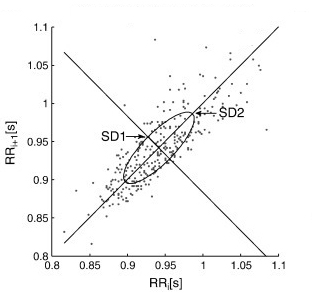
\includegraphics[scale=0.85]{latex_code/Figures_new/poincare2.jpg}
    \caption{Διάγραμμα \selectlanguage{english}Poincare\selectlanguage{greek}}
    \label{fig:poincare_plot}
\end{figure}


Όπως επίσης φαίνεται στο σχήμα, είναι σημειωμένες οι τυπικές αποκλίσεις \selectlanguage{english}SD1\selectlanguage{greek} και \selectlanguage{english}SD2\selectlanguage{greek} του συνόλου των σημείων από την μη κύρια και την κύρια διαγώνιο αντίστοιχα. Οι τυπικές αποκλίσεις αυτές είναι 2 από τα 4 χαρακτηριστικά που εξάγουμε από το συγκεκριμένο διάγραμμα. Τα υπόλοιπα 2 είναι η αναλογία $\frac{SD2}{SD1}$ των δύο τυπικών αποκλίσεων, καθώς και η επιφάνεια της έλλειψης που δημιουργείται από αυτές τις δύο τιμές, που βέβαια δίνεται από την τιμή $\pi \cdot SD1 \cdot SD2$.

\paragraph{\selectlanguage{english}Approximate Entropy\selectlanguage{greek}}

Μία πολύ σημαντική μετρική για την ανάλυσή μας, είναι η μετρική \selectlanguage{english}Approximate Entropy\selectlanguage{greek} (προσεγγιστική εντροπία) \cite{wikiAppEn}. Η προσεγγιστική εντροπία είναι μια στατιστική τεχνική με την οποία ποσοτικοποιούμε την κανονικότητα και την προβλεψιμότητα ενός σήματος. 

Ας πάρουμε για παράδειγμα την εξής χρονοσειρά : \{10, 20, 10, 20, 10, 20\}. Χρησιμοποιώντας τη μέση τιμή, την τυπική απόκλιση ή οποιασδήποτε τάξης ροπή, δεν μπορούμε να εκφράσουμε την επαναληπτικότητα και την κανονικότητα που εμφανίζει το μοτίβο αυτής της χρονοσειράς. 

Το στατιστικό μέγεθος που μπορεί να μας βοηθήσει να εντοπίσουμε την κανονικότητα ενός παρατηρούμενου μεγέθους είναι η εντροπία του. Ωστόσο, καθότι ο υπολογισμός της ακριβούς εντροπίας είναι συνήθως απαγορευτικά πολύπλοκος, αντί για την ακριβή εντροπία χρησιμοποιούμε μια προσέγγισή της. Ο αλγόριθμος που ακολουθεί για τον υπολογισμό αυτού του μεγέθους είναι μια επινόηση του μαθηματικού \selectlanguage{english}Steve M. Pincus\selectlanguage{greek}.

\begin{enumerate}
    \item Δημιουργούμε τη χρονοσειρά $u(1), u(2), ..., u(n)$ εισάγοντας το ΗΚΓ μας. Το μέγεθος των δεδομένων είναι ίσο με Ν.
    \item Εισάγουμε τις σταθερές $m$ και $r$. Η $m$ είναι μια ακέραια σταθερά που αναπαριστά το μήκος των συγκρινόμενων δεδομένων, και η $r$ είναι ένας πραγματικός αριθμός που εκφράζει το επίπεδο του φιλτραρίσματος, κάτι που θα φανεί καλύτερα στα επόμενα βήματα.
    \item Δημιουργούμε τα διανύσματα $\textbf{\selectlanguage{english}x\selectlanguage{greek}}(1), \textbf{\selectlanguage{english}x\selectlanguage{greek}}(2), ..., \textbf{\selectlanguage{english}x\selectlanguage{greek}}(N - m + 1)$, που ανήκουν στον $R^m$ πραγματικό χώρο, που ορίζεται από τα $\textbf{\selectlanguage{english}x\selectlanguage{greek}}(i) = [u(i), u(i + 1), ..., u(i + m - 1)] $.
    \item Χρησιμοποιούμε τη σειρά $\textbf{\selectlanguage{english}x\selectlanguage{greek}}(1), \textbf{\selectlanguage{english}x\selectlanguage{greek}}(2), ..., \textbf{\selectlanguage{english}x\selectlanguage{greek}}(N - m + 1)$ για να κατασκευάσουμε για κάθε $i, 1 \leq i \leq N -m + 1 : $
    $C^m_i(r) = $ (πλήθος των $x(j)$ τέτοιων ώστε $d[x(i), x(j)] \leq r) / (N - m + 1)$,
    όπου η απόσταση $d[x, x^*]$ ορίζεται ως $d[x,x^*] = max_a|u(a) - u^*(a)|.$
    
    Η παραπάνω εκδοχή της απόστασης μεταξύ δύο διανυσμάτων, δίνει ως αποτέλεσμα τη μέγιστη απόσταση μεταξύ δύο βαθμωτών τους διαστάσεων. Σημειώνεται ότι ο αλγάριθμος λαμβάνει υπόψη και την περίπτωση όπου $i = j$, στην οποία όπως γίνεται αντιληπτό η συνθήκη ελέγχου είναι πάντα αληθής. Αυτό συμβαίνει ούτως ώστε η είσοδος του λογάριθμου να μην είναι ποτέ μηδενική. Ωστόσο, όπως καταλαβαίνουμε, αυτό δημιουργεί μια μεροληπτική τάση υπέρ της κανονικότητας του σήματος.
    
    \item Ορίζουμε το μέγεθος $\Phi^m(r) = (N - m + 1)^{-1}\sum^{N - m + 1}_{i = 1}log(C^m_i(r))$, όπου $log$ είναι ο φυσικός λογάριθμος.
    
    \item Ορίζουμε τη μετρική \selectlanguage{english}Approximate Entropy\selectlanguage{greek} ως εξής: $ApEn = \Phi^m(r) - \Phi^{m+1}(r).$
\end{enumerate}

Η ερμηνεία της παραπάνω μετρικής είναι η εξής: Η παρουσία επαναλαμβανόμενων μοτίβων σε μια χρονσειρά την καθιστά πιο προβλέψιμη από ότι θα ήταν αν αυτά τα μοτίβα απουσιάζαν. Η προσεγγιστική εντροπία εκφράζει την πιθανότητα ορισμένα μοτίβα παρατηρήσεων να \emph{μην} ακολουθούνται από παρόμοια μοτίβα.

Συνεπώς, όσο μικρότερη είναι η τιμή αυτού του μέτρου, τόσο μεγαλύτερη είναι η προβλεψιμότητα του σήματος εισόδου.

Παρακάτω σημειώνονται ορισμένες παρατηρήσεις που συνοδεύουν τον αλγόριθμο.

\begin{itemize}
    \item Όπως εύκολα καταλαβαίνουμε από μια πρόχειρη ανάλυση του αλγορίθμου, η πολυπλοκότητά του είναι $O(N^2)$. Αυτός είναι και ο λόγος για τον οποίο δεν θα χρησιμοποιήσουμε σαν είσοδο για τον αλγόριθμο ολόκληρα ΗΚΓ, αλλά μόνο μικρά τμήματά τους, κάτι που θα αναλυθεί περαιτέρω στη συνέχεια.
    \item Ο αλγόριθμος εξαρτάται σημαντικά από το πλήθος των δειγμάτων που λαμβάνει ως είσοδο. Επομένως, είναι πολύ σημαντικό να υπάρχει συνέπεια μεταξύ των δεδομένων εκπαίδευσης και των δεδομένων ελέγχου.
    \item Είναι επίσης σημαντικό να υπάρχει συνέπεια όσον αφορά στο πλάτος των κυματομορφών που εισάγονται στον αλγόριθμο, δεδομένου ότι η παράμετρος $r$ διατηρείται σταθερή.
\end{itemize}

Με βάση τα παραπάνω, και γνωρίζοντας τους υπολογιστικούς περιορισμούς στους οποίους υπάγεται η παρούσα μελέτη, τέθηκαν οι εξής προδιαγραφές για κάθε σήμα που εισάγεται ούτως ώστε να εξαχθεί από αυτό η προσεγγιστική εντροπία:
\begin{itemize}
    \item Πριν την εισαγωγή του προς ανάλυση, το σήμα θα πρέπει να έχει κανονικοποιηθεί γραμμικά, ώστε η μέγιστη τιμή στα δείγματά του να είναι ίση με τη μονάδα. Αυτό γίνεται ούτως ώστε να υπάρχει μια συνέπεια απέναντι στη σταθερά $r$ που χρησιμοποιείται.
    \item Τα δείγματα που θα εισάγονται προς ανάλυση, θα πρέπει να έχουν προσεγγιστικά συχνότητα δειγματοληψίας 64 \selectlanguage{english}Hz\selectlanguage{greek} και διάρκεια 5 \selectlanguage{english}sec\selectlanguage{greek}. Αυτό γίνεται επίσης για λόγους συνέπειας, καθώς όπως αναφέρθηκε προηγουμένως το μέγεθος του δείγματος επηρεάζει σημαντικά το αποτέλεσμα των υπολογισμών. Σημειώνεται ότι επιλέχτηκε η συχνότητα 64 \selectlanguage{english}Hz\selectlanguage{greek} για τους εξής 3 λόγους: α) δεν είναι απαγορευτική υπολογιστικά η εφαρμογή του αλγορίθμου για διάστημα 5 δευτερολέπτων σε έναν επεξεργαστή κινητού β) η συντριπτική πλειοψηφία των συχνοτήτων δειγματοληψίας που συναντώνται διαρείται με τον αριθμό 64 προσεγγιστικά, οπότε μπορεί εύκολα να εφαρμοστεί υποδειγματοληψία για να μεταφερθεί το σήμα στην κατάλληλη μορφή γ) η συχνότητα των 64 \selectlanguage{english}Hz\selectlanguage{greek} διατηρεί τα βασικά χαρακτηριστικά της κυματομορφής του ΗΚΓ αναλλοίωτα.
    \item Η σταθερά $m$ επιλέχτηκε ίση με 2.
    \item Η σταθερά $r$ επιλέχτηκε ίση με 0.02 κατόπιν δοκιμών.
\end{itemize}

\paragraph{\selectlanguage{english}Sample Entropy\selectlanguage{greek}}

Η δειγματική εντροπία είναι μια εναλλακτική μετρική ποσοτικοποίησης της κανονικότητας και της προβλεψιμότητας ενός σήματος \cite{wikiSampEn}. Τα πλεονεκτήματα της συγκεκριμένης μετρικής έναντι της μετρικής \selectlanguage{english}Approximate Entropy\selectlanguage{greek} είναι αφενός η πιο εύκολη υλοποίηση, αφετέρου η μικρότερη συσχέτιση του αποτελέσματος με το μέγεθος του δείγματος. Στη συνέχεια θα παρουσιάσουμε τον αλγόριθμο με τον οποίο υπολογίζεται η παραπάνω μετρική.

\begin{enumerate}
    \item Δημιουργούμε τη χρονοσειρά $u(1), u(2), ..., u(n)$ εισάγοντας το ΗΚΓ μας. Το μέγεθος των δεδομένων είναι ίσο με Ν.
    \item Εισάγουμε τις σταθερές $m$ και $r$. Η $m$ είναι μια ακέραια σταθερά που αναπαριστά το μήκος των συγκρινόμενων δεδομένων, και η $r$ είναι ένας πραγματικός αριθμός που εκφράζει το επίπεδο του φιλτραρίσματος, κατά αναλογία με την προσεγγιστική εντροπία.
    \item Δημιουργούμε τα διανύσματα $\textbf{\selectlanguage{english}x\selectlanguage{greek}}_m(1), \textbf{\selectlanguage{english}x\selectlanguage{greek}}_m(2), ..., \textbf{\selectlanguage{english}x\selectlanguage{greek}}_m(N - m + 1)$, που ανήκουν στον $R^m$ πραγματικό χώρο, που ορίζεται από τα $\textbf{\selectlanguage{english}x\selectlanguage{greek}}(i) = [u(i), u(i + 1), ..., u(i + m - 1)] $.
    \item Ορίζουμε τη μεταβλητή $A_m = $ (πλήθος των ζευγαριών διανυσμάτων για τα οποία ισχύει $d[\textbf{\selectlanguage{english}x\selectlanguage{greek}}_m(i), \textbf{\selectlanguage{english}x\selectlanguage{greek}}_m(j)] < r$). Η συνάρτηση $d$ απόστασης, είναι η ίδια συνάρτηση που χρησιμοποιήθηκε στην προσεγγιστική εντροπία.
    \item Ορίζουμε τη μετρική \selectlanguage{english}Sample Entropy\selectlanguage{greek} ως εξής: $SampEn = -log\frac{A_{m+1}}{A_m}$.
\end{enumerate}

Από τον ορισμό της συνάρτησης απόστασης, είναι εμφανές ότι ισχύει $A_{m+1} \leq A_m$. Συνεπώς, το κλάσμα που εμφανίζεται στο λογάριθμο θα είναι μικρότερο της μονάδας. Στο μη πιθανό ενδεχόμενο που ένα εκ των $A_{m+1}, A_m$ είναι 0, ο αλγόριθμος έχει επιλεγεί να επιστρέφει μηδενική τιμή. Ωστόσο μπορούμε εύκολα να αντιληφθούμε, ότι με κατάλληλη επιλογή της παραμέτρου $r$, μπορεί η πιθανότητα εμφάνισης αυτής της περίπτωσης να μηδενιστεί.

Η ερμηνεία της συγκεκριμένη μετρικής είναι ίδια με την ερμηνεία της προσεγγιστικής εντροπίας. Και στην προκειμένη περίπτωση, το μικρότερο αποτέλεσμα αναπαριστά τη μεγαλύτερη κανονικότητα και προβλεψιμότητα.

Σχετικά με τον συγκεκριμένο αλγόριθμο, μπορούμε να κάνουμε τις εξής παρατηρήσεις:
 \begin{itemize}
     \item Παρόμοια με την προσεγγιστική εντροπία, η πολυπλοκότητά του είναι $O(N^2)$.
     \item Η τιμή του δεν εξαρτάται σε τόσο μεγάλο βαθμό από το μήκος του δείγματος. Και αυτό συμβαίνει γιατί στην προκειμένη περίπτωση απλά υπολογίζεται το συνολικό άθροισμα των σημείων που πληρούν τη συγκεκριμένη προϋπόθεση. Παρόλα αυτά, διενεργώνοντας έναν απλό έλεγχο, βλέπουμε ότι εφαρμόζοντας υποδειγματοληψίες διαφορετικής κλίμακας σε κάποιο σήμα εισόδου, παίρνουμε σημαντικά διαφορετικές τιμές. Επομένως, γίνεται αντιληπτό ότι οι κανόνες συνέπειας που εφαρμόστηκαν στην προσεγγιστική εντροπία.
     \item Παρομοίως, οφείλουμε να εφαρμόσουμε αντίστοιχους κανόνες αναφορικά με το πλάτος της κυματομορφής εισόδου.
 \end{itemize}
 
 Με βάση τα παραπάνω, καταλήγουμε στις εξής προδιαγραφές για τα σήματα εισόδου στον αλγόριθμο της δειγματικής εντροπίας:
 \begin{itemize}
     \item Τα δείγματα προς ανάλυση θα πρέπει να έχουν κανονικοποιηθεί γραμμικά ως προς το πλάτος, ούτως ώστε το μέγιστο πλάτος που εμφανίζεται να είναι ίσο με τη μονάδα.
     \item Τα δείγματα προς ανάλυση πρέπει να έχουν προσεγγιστικά συχνότητα δειγματοληψίας 64 \selectlanguage{english}Hz\selectlanguage{greek} και διάρκεια 5 \selectlanguage{english}sec\selectlanguage{greek}.
    \item Η σταθερά $m$ επιλέχτηκε ίση με 2.
    \item Η σταθερά $r$ επιλέχτηκε ίση με 0.02 κατόπιν δοκιμών.
 \end{itemize}
 
 




\clearpage
%\renewcommand\headrulewidth{0pt} % Size of the header rule
\setcounter{secnumdepth}{0}
\fancyhead[L]{}
\bibliographystyle{IEEEtran}
\selectlanguage{english}
\bibliography{Bibben.bib}
\clearpage
\fancyhead[L]{}
\setcounter{secnumdepth}{3}
\appendix
\section{Appendix}
% \subsection{Matlab script - "MyConverterModelling.m"}
% \lstinputlisting{MyConverterModelling.m}
% \subsection{Matlab function - "conv\_models.m"}
% \lstinputlisting{conv_modelsNew.m}
% \subsection{Matlab script - "MyConverterSimulink.m"}
% \lstinputlisting{MyConverterSimulink.m}
% \subsection{Simulink function block - "G{c}"}
% \lstinputlisting{Gc_Function.m}

\clearpage

\end{document}
